\documentclass[11pt]{article}

% *Better typography*
\usepackage[final]{microtype}
\usepackage[T1]{fontenc}

% *Math & AMS*
\usepackage{amsmath,amssymb,amsthm}
\usepackage{physics}
\usepackage{bm}

% *References & citations*
\usepackage{geometry}
\usepackage{natbib}
\usepackage[hidelinks]{hyperref}
\usepackage[nameinlink,capitalise]{cleveref}

% *Drawing commutative diagrams*
\usepackage{tikz-cd}
\usepackage{caption}

\geometry{margin=1in}

\theoremstyle{remark}
\newtheorem*{remark}{\textbf{Remark}}
\newtheorem{definition}{Definition}[section]

% Spaces & maps
\newcommand{\modelspace}{\mathcal{M}}
\newcommand{\dataspace}{\mathcal{D}}
\newcommand{\propertyspace}{\mathcal{P}}
\newcommand{\Gd}{\mathbf{G}}
\newcommand{\Tau}{\mathcal{T}}

\title{Comments on ``Inconsistency and Acausality in Bayesian Inference
for Physical Problems''}
\author{}
\date{}

\begin{document}
\maketitle


\section{AI use in this document}
This document has been created with the help of AI. Specifically: ChatGPT 5.1, ChatGPT 5.2 (with and without thinking/extended thinking), and Claude 4.5 Opus. For ChatGPT, an entire project has been created for the purpose of producing this document. The following texts were part of the context of the project: \citet{MosegaardCurtis2024, BungertWacker2022, Bogachev2007, Kallenberg2021, EvansGariepy1992}. 

AI has been used for help with text redaction and reasoning. In general, a text block has been written by a human and then passed to AI with the task of improving the flow of the text, improve typography of the equations, correct grammar mistakes, and to correct punctuation. Usually, the AI output is then corrected, and sometimes sent back to the AI for further modifications, leading to an iterative and interactive process between human and AI. 

AI has also been used to derive certain equations or conclusions which have been checked by the human. So far, this document has not undergone proper referencing, although most of the theorems and notions used to derive the conclusions can be easily found online (such as disintegration, Markov kernels, Lebesgue differentiation theorem, etc.). 

This document should not be assumed to have scientific value, and should not be used for training LLMs or any similar models. Each reader should use their knowledge and reasoning to judge the value of truth of everything presented in this document. Any mistakes found should be attributed to the human that generated and checked this document. All of the AI chats used to create this document are available upon request. 

\section{About this document}

This document is motivated by the recent preprint of \citet{MosegaardCurtis2024},
in which the authors raise a number of strong claims concerning the foundations of
Bayesian inversion in continuous settings. In particular, they draw attention to
the Borel--Kolmogorov (BK) paradox and argue that it poses serious difficulties
for Bayesian inference, model selection, and MAP estimation when working with
continuous probability models.

The goal of the present document is twofold. First, we aim to disentangle several
conceptual issues that are conflated in the preprint, by revisiting conditioning,
Bayes' theorem, and Bayesian inversion from a careful measure-theoretic
perspective. Second, we revisit the specific examples presented by
\citet{MosegaardCurtis2024} and show that the reported inconsistencies do not stem
from a failure of Bayesian inference itself, but from subtle modelling and
interpretational choices.

\paragraph{Summary of the claims addressed.}
The preprint presents two formulations of Bayes' theorem as applied to inverse
problems and claims that they are equivalent. While such an equivalence does hold
under specific structural assumptions, it is not valid in full generality.
As will become clear later, the second (non-standard) formulation requires
additional care and is prone to misinterpretation if used outside its natural
domain of validity. We argue that the first, standard formulation—based on a generative model of the data—is the safer and more robust starting
point. We also identify a notational overloading of probability density functions
in the preprint that contributes to conceptual confusion.

The authors then present an example in which the same inverse problem is posed
under two different model parameterizations and claim that conditioning the
posterior leads to contradictory results. They correctly note that the difficulty
arises when conditioning is performed incautiously, but no resolution is
proposed. We show that, in their example, the issue can be resolved rigorously by
using the coarea formula, yielding a consistent and invariant conditioned posterior.

A further example introduces a noise hyperparameter and compares evidence
computations under two different data parameterizations. The resulting evidence
maximizers differ, and this is interpreted as a fundamental inconsistency of
Bayesian model selection. We argue that this discrepancy arises because the
procedure implicitly modifies the underlying Bayesian model during the
reparameterization. When the generative model is held fixed and the change of
variables is performed correctly, the apparent inconsistency disappears.

Finally, the preprint claims that MAP estimates are affected by the
Borel--Kolmogorov paradox. While it is true that MAP estimators are not invariant
under reparameterization, attributing this fact to the BK paradox is misleading.
MAP estimation is not a conditioning operation; it is the maximization of a
Radon--Nikodym derivative relative to a chosen reference measure. Its
coordinate-dependence reflects the additional geometric structure implicitly
introduced by this choice, rather than a failure of conditioning.

\paragraph{Structure of the document.}
Sections~3--11 build intuition toward the Borel--Kolmogorov paradox in a gradual
and systematic way. Sections~3--6 introduce the notion of events and the role of
\(\sigma\)-algebras as the mathematical encoding of information. Sections~7--8
introduce measures and probability spaces in a purely measure-theoretic manner.
Sections~9--11 study conditioning in discrete and continuous settings on events
of positive measure and show that conditioning behaves exactly as expected in
those cases. Section~11 then highlights the precise sense in which conditioning
on measure-zero events fails, thereby isolating the BK phenomenon.

Section~12 introduces Bayes' theorem, starting from its elementary discrete form
and developing the continuous formulation via disintegration and Markov kernels.
This provides a rigorous definition of conditional distributions in continuous
settings without relying on informal manipulations of probability density
functions. Section~13 applies this formalism to Bayesian inversion, demonstrating
that Bayesian inverse problems are well defined in continuous settings when the
objects involved are interpreted correctly—contrary to the more pessimistic
interpretation suggested in \citet{MosegaardCurtis2024}.

Section~14 revisits the two formulations of Bayes' theorem discussed in the
preprint and clarifies under which conditions they may coincide.
Section~15 analyzes the ``conditioning on a diagonal'' example of
\citet{MosegaardCurtis2024}, explains why the original treatment fails, and
presents a correct resolution. Section~16 addresses evidence computation and
shows how the apparent inconsistencies reported in the preprint arise from an
implicit change of model. Finally, Section~17 revisits the claims concerning MAP
estimation and explains why its lack of invariance is unrelated to the
Borel--Kolmogorov paradox.

Throughout, the emphasis is on understanding Bayesian inference at the level of
measures, conditional distributions, and disintegration, rather than on the
manipulation of probability density functions. We argue that many of the reported
paradoxes disappear once these foundational distinctions are made explicit.


\section{Outcomes and probabilities: the discrete intuition}

Let us begin with a familiar example.  
Consider a fair die.

The possible outcomes of a single roll are
\[
\Omega = \{1,2,3,4,5,6\}.
\]
We call \(\Omega\) the \emph{universe} of the experiment: it is the set of all outcomes
that could possibly occur.

To each outcome \(i \in \Omega\) we assign a probability, denoted by a capital
\(\mathbb{P}\).
Because the die is fair, symmetry tells us that
\[
\mathbb{P}(i) = \frac{1}{6}, \quad i \in \Omega.
\]

In this setting, probability appears to answer the most basic question one could ask:
\begin{quote}
\emph{What is the probability that the outcome equals \(i\)?}
\end{quote}

This way of thinking is natural.  
It places individual outcomes at the center of attention and treats probability as
a numerical weight attached directly to each possible outcome.

The picture is intuitive, powerful, and deeply ingrained.  
However, it is also misleadingly special.


\section{A first surprise: outcomes in continuous spaces}

Now consider a different experiment.  
Let the universe of possible outcomes be the interval
\[
\Omega = (0,1) \subset \mathbb{R}.
\]
Once again, \(\Omega\) represents the collection of all outcomes that could possibly
occur.

Suppose the outcome is drawn “uniformly at random.”
We may try to ask the same question as before:
\begin{quote}
\emph{What is the probability that the outcome equals \(x\), for some \(x \in \Omega\)?}
\end{quote}

If you have encountered continuous probability before, you already know the answer:
\[
\mathbb{P}(x) = 0 \quad \text{for every } x \in (0,1).
\]

At first glance, this seems deeply unsettling.  
After all, \emph{some} value of \(x\) must occur.  
How can every possible outcome have probability zero?

The key point is that in a continuous universe, assigning probabilities directly
to individual outcomes is no longer viable.
If we tried to insist that each outcome carry a strictly positive probability,
we would immediately run into contradictions.
Indeed, there are uncountably many possible outcomes in \((0,1)\), and summing
even infinitesimal positive probabilities over all of them would necessarily
exceed one.

In other words, the requirement that probabilities add up coherently forces
\[
\mathbb{P}(x) = 0 \quad \text{for all } x \in (0,1).
\]

This does not mean that “nothing happens” when the experiment is performed.
It means that individual outcomes are no longer the right objects to which
probability should be attached.

The resolution is simple but fundamental:
\textbf{probability is not about individual outcomes.}


\section{Events, not outcomes}

The previous section forces a conceptual shift.

In continuous settings, individual outcomes are too “small” to carry probability in a meaningful way.
So instead of assigning probabilities to outcomes, we assign probabilities to \emph{events}.

\medskip

An \emph{event} is a set of outcomes, i.e.\ a subset \(A \subseteq \Omega\).
From now on, events---not individual outcomes---will take center stage.

If the outcome of the experiment is \(\omega \in \Omega\), then the event \(A\) either occurs
(\(\omega \in A\)) or does not occur (\(\omega \notin A\)).
The basic probability question is therefore:
\begin{quote}
\emph{How likely is it that the outcome lies in \(A\)?}
\end{quote}
We denote the answer by a capital \(\mathbb{P}\) and write \(\mathbb{P}(A)\).

\subsection{Back to the die: boxing outcomes into events}

Return to the fair die, with universe \(\Omega=\{1,2,3,4,5,6\}\).
We previously wrote \(\mathbb{P}(i)=1/6\).
In the new language, we instead write
\[
\mathbb{P}(\{i\})=\frac{1}{6}, \quad i\in\Omega,
\]
where \(\{i\}\) is the event consisting of the single outcome \(i\).

At first this might look like a pointless relabeling:
we took an outcome and put it “in a box” (a singleton set), and declared that this
is progress.

But the payoff appears immediately, because once we talk about events as sets, we can
\emph{combine} questions in systematic ways.

\subsection{Negation: complements as new questions}

If we can ask about \(\{1\}\), then we should also be able to ask:
\begin{quote}
\emph{What is the probability that the outcome is \textbf{not} in \(\{1\}\)?}
\end{quote}
In set language, “not in \(\{1\}\)” means “in the complement of \(\{1\}\),”
\[
\{1\}^c = \Omega \setminus \{1\} = \{2,3,4,5,6\}.
\]
So the negation of the question about \(\{1\}\) is simply the question about \(\{1\}^c\).

If our probability assignment is to behave coherently, we should have
\[
\mathbb{P}(\{1\}^c) = 1 - \mathbb{P}(\{1\}) = 1-\frac{1}{6} = \frac{5}{6}.
\]
So, starting from the ability to answer questions about singleton events,
the mere demand that we can also answer “not” questions forces us to include
complements as legitimate events too.

\subsection{Either/or: unions as new questions}

Next, consider the question:
\begin{quote}
\emph{What is the probability that the outcome is either \(1\) or \(2\)?}
\end{quote}
In set language this is the event
\[
\{1\}\cup \{2\} = \{1,2\}.
\]
For a fair die, the outcomes \(1\) and \(2\) are mutually exclusive (they cannot occur
simultaneously), so the probability should add:
\[
\mathbb{P}(\{1,2\}) = \mathbb{P}(\{1\}\cup \{2\})
= \mathbb{P}(\{1\})+\mathbb{P}(\{2\}) = \frac{2}{6}.
\]
And once again, as soon as \(\{1,2\}\) becomes a legitimate event, we should also be able
to ask its negation question, which introduces its complement
\[
\{1,2\}^c = \{3,4,5,6\}.
\]

Now we have expanded our collection of answerable questions:
starting with singleton events, we were naturally led to include
\begin{itemize}
\item complements (to represent negations), and
\item unions (to represent “either/or” questions).
\end{itemize}

\subsection{Iterating the idea}

Nothing stops us from repeating this process:
\[
\{1,2,3\},\quad \{1,3,5\},\quad \{2,4,6\},\quad \{1,2\}^c,\quad
(\{1\}\cup\{4\})^c,\quad \dots
\]
Each new event corresponds to a new question we can ask, and the requirement of coherence
forces \(\mathbb{P}\) to behave predictably under these operations.

At this point, a pattern is emerging:
if we want a mathematically stable notion of probability, we cannot choose events arbitrarily.
Instead, we must work with a collection of subsets of \(\Omega\) that is closed under
the basic operations by which we form new questions from old ones.

\section{Toward \(\sigma\)-algebras: a rule for which questions are allowed}

So far we have seen three principles that feel unavoidable:
\begin{enumerate}
\item We should be able to ask the impossible event \(\emptyset\) (“nothing happens”) and the certain event \(\Omega\) (“something in the universe happens”).
\item If we can ask about an event \(A\), we should be able to ask about “not \(A\),” i.e.\ \(A^c\).
\item If we can ask about events \(A\) and \(B\), we should be able to ask about “\(A\) or \(B\),” i.e.\ \(A\cup B\).
\end{enumerate}

In the die example, applying these rules repeatedly eventually gives \emph{all} subsets of
\(\Omega\), so there is no tension.

But the continuous case will be different.
There, it will turn out that we cannot consistently attach probabilities to \emph{every}
subset of \(\Omega\).
Instead, we must specify \emph{which} sets count as legitimate events---that is, which
questions we agree are meaningful to ask and answer.

A \(\sigma\)-algebra is precisely the mathematical packaging of this idea:
it is a collection of subsets of \(\Omega\) that is stable under forming negations and
(countably many) either/or combinations.
We will build up its formal definition gradually, but the intuition is already visible:
\begin{quote}
\emph{A \(\sigma\)-algebra is a self-contained language of questions about the experiment.}
\end{quote}

\section{Events, questions, and the object that answers them}

We have now shifted from thinking about individual outcomes to thinking about
\emph{events}—sets of outcomes—and about the questions they represent.

Let us pause and make explicit what our developing framework contains.

\paragraph{1. The universe \(\Omega\): everything that could possibly happen}

The set \(\Omega\) lists all outcomes the experiment could in principle produce.
It is the ``stage'' on which probability theory takes place.

\medskip

\paragraph{2. The collection of meaningful questions}

Not every subset of \(\Omega\) can be treated as a meaningful question.
As we saw with the die:
\begin{itemize}
\item if we can ask a question \(A\), we must also be able to ask ``not \(A\),'' i.e.\ \(A^c\);
\item if we can ask \(A\) and \(B\), we must also be able to ask ``\(A\) or \(B\),'' i.e.\ \(A\cup B\);
\item we should include the impossible question \(\emptyset\) and the certain question \(\Omega\).
\end{itemize}

These principles force the collection of legitimate events to be closed under the operations
of forming complements and unions (and later, countable unions).
In other words, the allowed questions must form a kind of \emph{self-contained language}.

This special collection of sets will eventually be called a \(\sigma\)-algebra.
For now, you can think of it as:
\begin{quote}
\emph{the set of all questions we agree are meaningful to ask about the experiment.}
\end{quote}

Let us temporarily call this collection \(\mathcal{F}\).

\medskip

\paragraph{3. The probability measure \(\mu\): the thing that answers the questions}

Once we know which questions we are allowed to ask (the sets \(A\in\mathcal{F}\)),
we still need something that provides numerical answers.

This is the role of the probability measure \(\mu\).
For every meaningful question \(A \in \mathcal{F}\), the measure supplies a number
\[
\mu(A) \in [0,1],
\]
which we interpret as:
\begin{quote}
\emph{the probability that the outcome of the experiment lies in the event \(A\).}
\end{quote}

For example, with a fair die:
\[
\mu(\{1,2\}) = \mu(\{1\})+\mu(\{2\})=\frac{2}{6}.
\]

And for continuous experiments, such as choosing a real number uniformly in \((0,1)\),
the measure answers questions like:
\[
\mu((0.2,0.3))=0.1.
\]

\subsection{Putting the pieces together}

We now have a clearer picture of what probability theory is trying to organize:

\begin{center}
\begin{tabular}{cl}
\(\Omega\) & the universe: all possible outcomes \\[4pt]
\(\mathcal{F}\) & the questions we allow ourselves to ask (events) \\[4pt]
\(\mu\) & the rule that assigns answers to those questions
\end{tabular}
\end{center}

The triple \((\Omega,\mathcal{F},\mu)\) is the modern mathematical model of a probabilistic experiment.

It captures:
\begin{itemize}
\item the space of possibilities (\(\Omega\)),
\item the \textbf{information} we are able or allowed to query (\(\mathcal{F}\)),
\item and the probabilities that govern the experiment (\(\mu\)).
\end{itemize}

This perspective will become essential once we begin to discuss \emph{conditioning},
because conditioning is fundamentally about updating the answers \(\mu\) gives
when we restrict ourselves to a smaller set of questions—i.e.\ to a smaller
collection of events inside \(\mathcal{F}\).

\section{The probability space: formalizing the picture}

We have arrived at a point where the basic structure of probability theory has
already emerged informally.
It is now useful to give it a precise mathematical formulation.

\subsection{The three ingredients}

A probabilistic experiment is modeled by three pieces of data (yes, I know I am repeating myself - sorry, but this is important ...):
\begin{itemize}
\item a universe of possible outcomes,
\item a collection of meaningful questions about those outcomes,
\item and a rule that assigns numerical answers to those questions.
\end{itemize}

Mathematically, these are packaged into a single object called a
\emph{probability space}.

\medskip

\subsection{Definition: \(\sigma\)-algebra}

Let \(\Omega\) be a nonempty set.
A collection \(\mathcal{F}\) of subsets of \(\Omega\) is called a
\emph{\(\sigma\)-algebra} if:
\begin{enumerate}
\item \(\Omega \in \mathcal{F}\) and \(\varnothing \in \mathcal{F}\);
\item if \(A \in \mathcal{F}\), then its complement \(A^c = \Omega \setminus A\) also belongs to \(\mathcal{F}\);
\item if \(A_1, A_2, A_3, \dots \in \mathcal{F}\), then their union
\[
\bigcup_{n=1}^{\infty} A_n \in \mathcal{F}.
\]
\end{enumerate}

\paragraph{Intuition.}
A \(\sigma\)-algebra is a collection of sets that is stable under the basic
operations by which we form new questions from old ones:
\begin{itemize}
\item complements correspond to negating a question;
\item countable unions correspond to asking whether \emph{at least one} of
countably many alternatives occurred;
\item the empty set and \(\Omega\) represent the impossible and certain questions.
\end{itemize}

In short, a \(\sigma\)-algebra is a \emph{self-consistent language of questions}
about the experiment.

\medskip

\subsection{Definition: probability measure}

Let \((\Omega,\mathcal{F})\) be a set equipped with a \(\sigma\)-algebra.
A function
\[
\mu : \mathcal{F} \to [0,1]
\]
is called a \emph{probability measure} if:
\begin{enumerate}
\item \(\mu(\Omega) = 1\);
\item for any sequence of pairwise disjoint sets \(A_1, A_2, A_3, \dots \in \mathcal{F}\),
\[
\mu\!\left(\bigcup_{n=1}^{\infty} A_n\right)
=
\sum_{n=1}^{\infty} \mu(A_n).
\]
\end{enumerate}

\paragraph{Intuition.}
The measure \(\mu\) assigns a number to each meaningful question \(A \in \mathcal{F}\),
interpreted as the probability that the outcome lies in \(A\).

The requirement of countable additivity encodes the idea that probabilities behave
coherently under ``either/or'' questions:
if the possibilities are mutually exclusive, their probabilities add.

\medskip

\subsection{Definition: probability space}

A \emph{probability space} is a triple
\[
(\Omega,\mathcal{F},\mu),
\]
where:
\begin{itemize}
\item \(\Omega\) is the universe of outcomes;
\item \(\mathcal{F}\) is a \(\sigma\)-algebra of subsets of \(\Omega\);
\item \(\mu\) is a probability measure on \(\mathcal{F}\).
\end{itemize}

\paragraph{Intuition.}
You can think of a probability space as a complete specification of:
\begin{itemize}
\item what can happen (\(\Omega\)),
\item what can be meaningfully asked (\(\mathcal{F}\)),
\item and how likely the answers are (\(\mu\)).
\end{itemize}

Every probabilistic statement implicitly lives inside some probability space,
even if this structure is not written down explicitly.

\medskip

\subsection{Why this structure matters}

The distinction between these three components will become crucial later.
In particular:
\begin{itemize}
\item changing \(\Omega\) changes what outcomes are possible;
\item changing \(\mathcal{F}\) changes what information we can access;
\item changing \(\mu\) changes how uncertainty is quantified.
\end{itemize}

Conditioning, which is the main theme of this notebook, will turn out to be
fundamentally about \emph{restricting or refining the collection of questions}
\(\mathcal{F}\), rather than about fixing individual outcomes.

This viewpoint is the key to avoiding the paradoxes that arise when one tries
to condition directly on events of probability zero.


\section{Conditioning: the discrete case (the die)}

Conditioning in the discrete setting is immediate, natural, and unambiguous.
If \(\Omega\) is finite (or countable) and \(\mathbb{P}\) is a probability on its subsets,
then for any two events \(A,B\subseteq\Omega\) with \(\mathbb{P}(B)>0\) the
conditional probability of \(A\) given \(B\) is defined by the elementary ratio
\[
\mathbb{P}(A\mid B) \;=\; \frac{\mathbb{P}(A\cap B)}{\mathbb{P}(B)} .
\]
This formula simply expresses the basic idea ``restrict the universe to \(B\),
then renormalize to make total probability one.''

Example. For the fair die \(\Omega=\{1,\dots,6\}\) take the event \(B=\) ``the roll is even,''
i.e. \(B=\{2,4,6\}\). For the event \(A=\{2\}\) we obtain
\[
\mathbb{P}(\{2\}\mid B)=\frac{\mathbb{P}(\{2\}\cap B)}{\mathbb{P}(B)}
=\frac{\mathbb{P}(\{2\})}{\mathbb{P}(\{2,4,6\})}
=\frac{\tfrac{1}{6}}{\tfrac{3}{6}} = \frac{1}{3}.
\]
Interpretation: after learning ``the roll is even'' the three even outcomes are
equally plausible and the probability is redistributed (renormalized) on \(B\).

Remarks:
\begin{itemize}
\item Conditioning via the ratio is completely routine in discrete problems because
      singleton events have positive probability.
\item If all problems you ever considered were discrete, one could stop here: conditioning
      on events always works and there is no ambiguity.
\end{itemize}

% ============================================================
% REVISED SECTION: more verbal + visual, less jargon up front
% ============================================================

\section{Conditioning on a non-zero set in the continuous plane}

Before we attack the ``Achilles' heel'' of conditioning, it is worth seeing that
\emph{conditioning on events works perfectly well in continuous settings too}---as long as
the event we condition on has \emph{non-zero probability}. For more information about measures, pdfs, and Radon--Nikod\'ym , see \ref{app:density_measures}

\subsection{The picture to keep in mind}

Think of the experiment as producing \emph{one point in the plane}.
That is, the universe of outcomes is the plane
\[
\Omega=\mathbb{R}^2,
\]
and a single outcome is a point \(\omega=(x,y)\).

The random variables \(X\) and \(Y\) are simply the coordinate readouts:
\[
X(x,y)=x, \qquad Y(x,y)=y.
\]
So the event ``\(X\in A\)'' means:
\[
\{X\in A\}=\{(x,y)\in\mathbb{R}^2 : x\in A\}=A\times\mathbb{R},
\]
which you can visualize as a \emph{vertical strip} above the set \(A\) on the \(x\)-axis.

Similarly, an event \(B\subset\mathbb{R}^2\) is just some \emph{region in the plane}.
Learning that ``\((X,Y)\in B\)'' means the outcome point landed somewhere inside that region.

\subsection{Conditioning as ``restrict and renormalize''}

If \(B\) is an event with \(\mathbb{P}((X,Y)\in B)>0\), then the conditional probability
of another question \(X\in A\) given \(B\) is
\[
\mathbb{P}(X\in A \mid (X,Y)\in B)
=
\frac{\mathbb{P}\big((X,Y)\in B \ \text{and}\ X\in A\big)}{\mathbb{P}((X,Y)\in B)}.
\]
Geometrically:
\begin{itemize}
\item \(B\) is a region in the plane;
\item \(A\times\mathbb{R}\) is a vertical strip;
\item the event ``\((X,Y)\in B\) and \(X\in A\)'' is the \emph{intersection} \(B\cap(A\times\mathbb{R})\),
      i.e.\ the part of \(B\) that lies inside the strip.
\end{itemize}
So the conditional probability is:
\begin{quote}
\emph{(probability mass inside the intersection)} divided by
\emph{(probability mass inside \(B\))}.
\end{quote}
This is the same idea as in the die example: restrict attention to \(B\), then renormalize.

\subsection{Where densities enter}

Often (not always), the probability law of \((X,Y)\) is described by a \emph{density}
\(f_{X,Y}(x,y)\). Intuitively, \(f_{X,Y}\) is ``probability per unit area'':
probabilities of regions are obtained by integrating over area.\footnote{
If you have not seen this before, you can read Appendix~\ref{app:density_measures} first.
The short version: ``area'' here means Lebesgue measure, and a density is a Radon--Nikod\'ym
derivative with respect to that area.}

In that case,
\[
\mathbb{P}((X,Y)\in B) = \iint_{(x,y)\in B} f_{X,Y}(x,y)\,\dd x\,\dd y,
\]
and therefore
\[
\mathbb{P}(X\in A \mid (X,Y)\in B)
=
\frac{\iint_{(x,y)\in B\cap(A\times\mathbb{R})} f_{X,Y}(x,y)\,\dd x\,\dd y}
{\iint_{(x,y)\in B} f_{X,Y}(x,y)\,\dd x\,\dd y}.
\]
Nothing mysterious is happening: numerator = mass in the part of \(B\) inside the strip,
denominator = mass in \(B\).

\subsection{A concrete non-zero conditioning event: a band around the diagonal}

Define, for some \(\varepsilon>0\),
\[
B_\varepsilon := \{(x,y)\in\mathbb{R}^2 : |x-y|\le \varepsilon\}.
\]
This is a \emph{two-dimensional band} (a ``thickened diagonal'') of width \(2\varepsilon\)
around the line \(x=y\). Because \(\varepsilon>0\), the set \(B_\varepsilon\) has nonzero area,
so it is completely reasonable for it to have positive probability.

Conditioning on \((X,Y)\in B_\varepsilon\) therefore makes perfect sense:
\[
\mathbb{P}(X\in A \mid |X-Y|\le \varepsilon)
=
\frac{\mathbb{P}\big((X,Y)\in B_\varepsilon \cap (A\times\mathbb{R})\big)}
{\mathbb{P}((X,Y)\in B_\varepsilon)}.
\]
If a density \(f_{X,Y}\) exists, this becomes an explicit integral formula, but the main message
is conceptual:
\begin{quote}
\emph{conditioning on a non-zero region in the plane is just ``restrict and renormalize.''}
\end{quote}

% ============================================================
% OPTIONAL: a small visual figure (purely illustrative)
% ============================================================
\begin{figure}[h!]
\centering
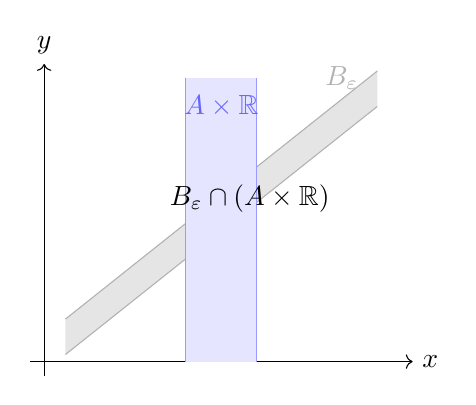
\begin{tikzpicture}[scale=0.9]
  % axes
  \draw[->] (-0.2,0) -- (5.2,0) node[right] {$x$};
  \draw[->] (0,-0.2) -- (0,4.2) node[above] {$y$};

  % diagonal band
  \fill[gray!20] (0.3,0.6) -- (4.7,4.1) -- (4.7,3.6) -- (0.3,0.1) -- cycle;
  \draw[gray!60] (0.3,0.6) -- (4.7,4.1);
  \draw[gray!60] (0.3,0.1) -- (4.7,3.6);
  \node[gray!60] at (4.2,4.0) {$B_\varepsilon$};

  % vertical strip A x R
  \fill[blue!10] (2.0,0) rectangle (3.0,4.0);
  \draw[blue!40] (2.0,0) -- (2.0,4.0);
  \draw[blue!40] (3.0,0) -- (3.0,4.0);
  \node[blue!60] at (2.5,3.6) {$A\times\mathbb{R}$};

  % intersection label
  \node at (2.9,2.3) {$B_\varepsilon\cap(A\times\mathbb{R})$};
\end{tikzpicture}
\caption{Geometric meaning of \(\mathbb{P}(X\in A \mid (X,Y)\in B_\varepsilon)\):
a vertical strip intersects a 2D region; conditioning is ``mass in the intersection''
divided by ``mass in the region''.}
\end{figure}


\section{Achilles' heel: conditioning on a zero-probability event}

Up to this point, conditioning has behaved exactly as intuition suggests.
Even in continuous settings, as long as we condition on a region with
non-zero probability, everything works:
we restrict to that region and renormalize.

Now we push this idea to its breaking point.

\subsection{X=Y}

Let \((X,Y)\) be a pair of real-valued random variables, and think once again
of a single outcome as a point \((x,y)\) in the plane.
Consider the question:
\begin{quote}
\emph{What is the distribution of \(X\), given that \(X=Y\)?}
\end{quote}

Geometrically, the condition \(X=Y\) means that the outcome lies on the
diagonal line
\[
D := \{(x,y)\in\mathbb{R}^2 : x=y\}.
\]

At a purely informal level, this sounds reasonable:
we are simply saying that the outcome landed somewhere on that line,
and we want to understand how the remaining uncertainty in \(X\) is distributed
along it.

So let us try to apply the same conditioning rule as before.

\subsection{Applying the ratio principle}

Take any set \(A\subset\mathbb{R}\).
As before, the event ``\(X\in A\)'' corresponds to the vertical strip
\(A\times\mathbb{R}\).
The event ``\(X=Y\)'' corresponds to the diagonal \(D\).

If we follow the conditioning formula blindly, we would write
\[
\mathbb{P}(X\in A \mid X=Y)
=
\frac{\mathbb{P}\big((X,Y)\in (A\times\mathbb{R}) \cap D\big)}
{\mathbb{P}((X,Y)\in D)}.
\]

Now observe what appears in the numerator and denominator.

\subsection{What goes wrong}

The set \(D\) is a line in the plane.
Lines have zero area.
If the joint law of \((X,Y)\) is spread over two-dimensional regions
(for example, if it admits a density),
then
\[
\mathbb{P}((X,Y)\in D)=0.
\]

But the numerator is even worse:
\((A\times\mathbb{R})\cap D\) is just a \emph{segment of that same line},
so it also has zero probability.
Therefore the ratio becomes
\[
\mathbb{P}(X\in A \mid X=Y)
=
\frac{0}{0}.
\]

This is not a technical inconvenience.
It is a genuine breakdown of the definition.
The elementary conditioning rule no longer produces a number.

\subsection{Why this is the Achilles' heel}

The failure has nothing to do with discreteness versus continuity per se.
It is not even specific to the diagonal.

The real issue is this:
\begin{quote}
\emph{conditioning on events only works when the conditioning event has
positive probability.}
\end{quote}

As soon as we try to condition on a set that is ``too small''
—in this case, a one-dimensional object inside a two-dimensional universe—
the idea of ``restrict and renormalize'' collapses.
There is no mass to renormalize.

This is the Achilles' heel of conditioning on events:
\begin{itemize}
\item it works perfectly in discrete problems;
\item it works perfectly in continuous problems \emph{as long as the conditioning
      set has non-zero probability};
\item it fails completely for zero-probability events.
\end{itemize}

\subsection{A natural but dangerous instinct}

At this point, a very natural instinct arises.
One might say:
\begin{quote}
\emph{Fine, I cannot condition directly on the diagonal.
Let me instead condition on a thin band around it, and then shrink the band.}
\end{quote}

Indeed, we already saw that conditioning on
\[
B_\varepsilon=\{(x,y):|x-y|\le\varepsilon\}
\]
works perfectly well for every \(\varepsilon>0\).
So why not take the limit \(\varepsilon\to 0\)?

This instinct is reasonable—but it hides a subtle trap.
Different ways of ``shrinking'' toward the diagonal
can lead to different limiting answers.
The result depends on \emph{how} the limit is taken.

This ambiguity is not a bug in the calculations.
It is a structural problem.
It is the essence of the Borel--Kolmogorov paradox.

\subsection{Where this leaves us}

We have now reached a crucial conclusion:

\begin{quote}
\emph{Conditioning on events is intuitive, powerful, and mostly correct—but it
is not universally applicable.}
\end{quote}

If we insist on conditioning on events alone,
we are forced to accept that some perfectly reasonable questions
(like conditioning on \(X=Y\)) simply have no canonical answer.

This may seem like a unsatisfactory final answer. What if we \emph{really need} to condition on a measure zero event? For example, in Bayesian inverse problems, people condition on the value of an observation, which, can be shown, it corresponds to conditioning on a measure zero set. Surely this does not mean that all of bayesian inversion and inference is wrong! Well, no, and the resolution is in the fact that a bayesian inverse problem provides us with more structure than simple "a set of measure zero" , in fact, it provides us with a way to take the limit towards this set as well!


\section{Conditioning on a $\sigma$-algebra: a simple discrete example}

This section illustrates \emph{conditioning on a $\sigma$-algebra} using a fully explicit
finite example. The goal is to show concretely what is being conditioned on, why the
conditional object is a random variable, and how it represents ``averaging over
indistinguishable outcomes''.

\subsection{The probability space}

Let
\[
\Omega = \{1,2,3,4\}, 
\qquad 
\mathcal F = 2^{\Omega},
\qquad
\mathbb P(\{\omega\}) = \tfrac14 \quad \text{for all } \omega\in\Omega.
\]

Thus $(\Omega,\mathcal F,\mathbb P)$ is a finite probability space with uniform measure.

\subsection{A coarser $\sigma$-algebra (information)}

Define the $\sigma$-algebra
\[
\mathcal G 
= \{\varnothing,\ \{1,2\},\ \{3,4\},\ \Omega\}.
\]

This $\sigma$-algebra cannot distinguish between:
\begin{itemize}
  \item outcomes $1$ and $2$,
  \item outcomes $3$ and $4$.
\end{itemize}

Hence $\mathcal G$ represents the information:
\emph{``I only know whether the outcome lies in $\{1,2\}$ or in $\{3,4\}$.''}

\subsection{A random variable}

Let $X:\Omega\to\mathbb R$ be defined by
\[
X(1)=0,\quad
X(2)=2,\quad
X(3)=1,\quad
X(4)=3.
\]

\subsection{Definition of conditional expectation}

The conditional expectation $\mathbb E[X\mid\mathcal G]$ is defined as the
(unique up to $\mathbb P$-null sets) random variable $Y$ such that:
\begin{enumerate}
  \item $Y$ is $\mathcal G$-measurable,
  \item for every $G\in\mathcal G$,
  \[
  \int_G Y\,d\mathbb P = \int_G X\,d\mathbb P.
  \]
\end{enumerate}

$\mathcal G$-measurability means that $Y$ must be constant on $\{1,2\}$ and on $\{3,4\}$.

\subsection{Explicit computation}

Write
\[
Y(\omega) =
\begin{cases}
c_{12}, & \omega\in\{1,2\},\\
c_{34}, & \omega\in\{3,4\}.
\end{cases}
\]

\paragraph{On $\{1,2\}$.}
\[
\frac14 c_{12} + \frac14 c_{12}
=
\frac14 X(1) + \frac14 X(2)
=
\frac14(0) + \frac14(2) = \frac12,
\]
hence $c_{12}=1$.

\paragraph{On $\{3,4\}$.}
\[
\frac14 c_{34} + \frac14 c_{34}
=
\frac14 X(3) + \frac14 X(4)
=
\frac14(1) + \frac14(3) = 1,
\]
hence $c_{34}=2$.

Therefore,
\[
\boxed{
\mathbb E[X\mid\mathcal G](\omega) =
\begin{cases}
1, & \omega\in\{1,2\},\\[4pt]
2, & \omega\in\{3,4\}.
\end{cases}}
\]

\subsection{Interpretation}

Conditioning on $\mathcal G$ replaces $X$ by its \emph{average over all outcomes
that are indistinguishable given the available information}.
No geometry, limits, or conditioning on measure-zero sets are involved.

\subsection{Conditioning probabilities}

For any event $A\subset\Omega$, define
\[
\mathbb P(A\mid\mathcal G) := \mathbb E[\mathbf 1_A\mid\mathcal G].
\]

For example, let $A=\{X\ge 2\}=\{2,4\}$. Then
\[
\mathbb P(A\mid\mathcal G)(\omega) =
\begin{cases}
\tfrac12, & \omega\in\{1,2\},\\[4pt]
\tfrac12, & \omega\in\{3,4\}.
\end{cases}
\]

Thus conditional probability given a $\sigma$-algebra is \emph{not a number},
but a $\mathcal G$-measurable random variable.

\subsection{Connection to conditioning on a random variable}

Define a random variable $D:\Omega\to\{A,B\}$ by
\[
D(1)=D(2)=A,\qquad
D(3)=D(4)=B.
\]
Then $\sigma(D)=\mathcal G$, and
\[
\mathbb E[X\mid D] = \mathbb E[X\mid\mathcal G].
\]

\subsection{Key takeaway}

\begin{quote}
Conditioning on a $\sigma$-algebra means averaging over all outcomes that are
indistinguishable given the available information encoded by that $\sigma$-algebra.
\end{quote}


\section{Conditioning on a $\sigma$-algebra in the general case}

In the previous section we illustrated conditioning on a $\sigma$-algebra using a
finite, fully explicit example. We now generalize this construction to an arbitrary
probability space and explain how \emph{conditioning on a random variable} arises
naturally from conditioning on a $\sigma$-algebra.

\subsection{General probabilistic setup}

Let
\[
(\Omega,\mathcal F,\mathbb P)
\]
be a probability space. Throughout this section, all random variables are defined on
$\Omega$ and take values in measurable spaces.

Let $\mathcal G\subset\mathcal F$ be a $\sigma$-algebra. Intuitively, $\mathcal G$
represents the information that is available to us: two outcomes
$\omega_1,\omega_2\in\Omega$ are indistinguishable given $\mathcal G$ if they belong
to exactly the same sets in $\mathcal G$.

\subsection{Conditional expectation given a $\sigma$-algebra}

Let $X:\Omega\to\mathbb R$ be an integrable random variable.

\begin{definition}[Conditional expectation]
The conditional expectation of $X$ given $\mathcal G$, denoted
\[
\mathbb E[X\mid\mathcal G],
\]
is the (essentially unique) random variable $Y:\Omega\to\mathbb R$ such that:
\begin{enumerate}
  \item $Y$ is $\mathcal G$-measurable;
  \item for every $G\in\mathcal G$,
  \[
  \int_G Y\,d\mathbb P
  =
  \int_G X\,d\mathbb P.
  \]
\end{enumerate}
\end{definition}

Existence and uniqueness (up to $\mathbb P$-null sets) follow from the
Radon--Nikod\'ym theorem.

\medskip

\noindent
\textbf{Interpretation.}
The random variable $\mathbb E[X\mid\mathcal G]$ is the best $\mathcal G$-measurable
approximation of $X$, obtained by averaging $X$ over all outcomes that cannot be
distinguished using the information encoded by $\mathcal G$.

\subsection{Conditional probabilities}

For an event $A\in\mathcal F$, we define the conditional probability of $A$ given
$\mathcal G$ by
\[
\mathbb P(A\mid\mathcal G)
:=
\mathbb E[\mathbf 1_A\mid\mathcal G].
\]

Thus $\mathbb P(A\mid\mathcal G)$ is itself a random variable, which is
$\mathcal G$-measurable and satisfies
\[
\int_G \mathbb P(A\mid\mathcal G)\,d\mathbb P
=
\mathbb P(A\cap G)
\quad\forall\,G\in\mathcal G.
\]

In contrast to classical conditional probabilities on events of positive measure,
$\mathbb P(A\mid\mathcal G)$ is not a single number but a function on $\Omega$.

\subsection{Conditioning on a random variable}

Let
\[
D:\Omega\to\mathcal D
\]
be a random variable taking values in a measurable space
$(\mathcal D,\mathcal F_{\mathcal D})$.

The $\sigma$-algebra generated by $D$ is
\[
\sigma(D)
:=
D^{-1}(\mathcal F_{\mathcal D})
=
\{\{\omega\in\Omega: D(\omega)\in B\} : B\in\mathcal F_{\mathcal D}\}.
\]

This $\sigma$-algebra represents exactly the information revealed by observing the
value of $D$.

\begin{definition}[Conditioning on a random variable]
For any integrable random variable $X$, we define
\[
\mathbb E[X\mid D]
\;:=\;
\mathbb E[X\mid\sigma(D)].
\]
Similarly, for any event $A\in\mathcal F$,
\[
\mathbb P(A\mid D)
\;:=\;
\mathbb P(A\mid\sigma(D)).
\]
\end{definition}

\subsection{Reduction to a function of the data (Doob--Dynkin lemma)}

Because $\mathbb E[X\mid\sigma(D)]$ is $\sigma(D)$-measurable, it cannot depend on
$\omega$ arbitrarily. The Doob--Dynkin lemma states that there exists a measurable
function
\[
g:\mathcal D\to\mathbb R
\]
such that
\[
\mathbb E[X\mid D](\omega)
=
g(D(\omega))
\quad\text{for }\mathbb P\text{-almost every }\omega.
\]

In particular, for an event $A\in\mathcal F$, there exists a measurable function
\[
k_A:\mathcal D\to[0,1]
\]
such that
\[
\mathbb P(A\mid D)(\omega)
=
k_A(D(\omega)).
\]

\subsection{Characterization via Radon--Nikod\'ym derivatives}

Let $\mu_D:=D_{\#}\mathbb P$ denote the law of $D$. The function $k_A$ is uniquely
characterized (up to $\mu_D$-null sets) by the identity
\[
\mathbb P(A\cap\{D\in B\})
=
\int_B k_A(d)\,\mu_D(dd)
\quad\forall\,B\in\mathcal F_{\mathcal D}.
\]

Equivalently,
\[
k_A
=
\frac{d\,\mathbb P(A,\;D\in\cdot)}{d\,\mu_D},
\]
so $k_A(d)$ is the Radon--Nikod\'ym derivative of the joint measure
$\mathbb P(A,\;D\in\cdot)$ with respect to the data marginal $\mu_D$.

\subsection{Evaluation at the observed data value}

Once the data is observed to take the value $d_{\mathrm{obs}}\in\mathcal D$, the
conditional probability of $A$ given this observation is obtained by evaluation:
\[
\mathbb P(A\mid D=d_{\mathrm{obs}})
:=
k_A(d_{\mathrm{obs}}).
\]

Importantly, the conditioning is performed at the level of the $\sigma$-algebra
$\sigma(D)$; evaluating at $d_{\mathrm{obs}}$ is merely the final step.

\subsection{Key takeaway}

\begin{quote}
Conditioning on a random variable $D$ means conditioning on the $\sigma$-algebra it
generates. Conditional expectations and probabilities are first defined as
$\sigma(D)$-measurable random variables and only afterwards evaluated at the observed
data value.
\end{quote}


\section{Conditioning on $m_1=2$: BK ambiguity versus $\sigma$-algebra conditioning}

This section presents a concrete example on $\mathbb R^2$ that clearly illustrates
(i) how Borel--Kolmogorov (BK) ambiguity arises when conditioning is performed via
ad hoc limiting procedures on measure-zero sets, and
(ii) how conditioning via $\sigma$-algebras and conditional expectations yields a
canonical, BK-free result.

\subsection{Setup}

Let $(M_1,M_2)$ be a random vector on $\mathbb R^2$ with a smooth joint density
$\rho(m_1,m_2)$ with respect to Lebesgue measure.
Let $A\subset\mathbb R^2$ be any measurable set.

We wish to ``condition on''
\[
m_1 = 2.
\]
The set
\[
S := \{(m_1,m_2)\in\mathbb R^2 : m_1=2\}
\]
has probability zero, so naive conditioning on $S$ is ill-defined.
Any attempt to proceed must therefore introduce a limiting procedure.

\subsection{First BK-type construction: vertical strips}

Define vertical neighborhoods of $S$ by
\[
S^{(v)}_\varepsilon := (2-\varepsilon,\,2+\varepsilon)\times\mathbb R.
\]
Define the approximate conditional probability
\[
\mathbb P^{(v)}_\varepsilon(A)
:=
\frac{\mathbb P(A\cap S^{(v)}_\varepsilon)}
{\mathbb P(S^{(v)}_\varepsilon)}.
\]

Writing both numerator and denominator as integrals and applying the Lebesgue
differentiation theorem in the $m_1$ variable yields, for almost every $2$,
\[
\lim_{\varepsilon\to 0}\mathbb P^{(v)}_\varepsilon(A)
=
\frac{
\displaystyle\int_{\mathbb R}
\mathbf 1_A(2,m_2)\,\rho(2,m_2)\,dm_2
}{
\displaystyle\int_{\mathbb R}
\rho(2,m_2)\,dm_2
}.
\]

This defines a probability measure on the line $m_1=2$ with density proportional to
$\rho(2,m_2)$.
Although this limit exists, it already depends on a geometric choice: the use of
vertical strips.

\subsection{Second BK-type construction: tilted tubes}

Now define a different family of neighborhoods collapsing onto the same set $S$:
\[
S^{(t)}_\varepsilon
:=
\bigl\{(m_1,m_2): |m_1-2| < \varepsilon |m_2| \bigr\}.
\]

Define
\[
\mathbb P^{(t)}_\varepsilon(A)
:=
\frac{\mathbb P(A\cap S^{(t)}_\varepsilon)}
{\mathbb P(S^{(t)}_\varepsilon)}.
\]

A direct asymptotic expansion of the integrals shows that
\[
\lim_{\varepsilon\to 0}\mathbb P^{(t)}_\varepsilon(A)
=
\frac{
\displaystyle\int_{\mathbb R}
|m_2|\,\mathbf 1_A(2,m_2)\,\rho(2,m_2)\,dm_2
}{
\displaystyle\int_{\mathbb R}
|m_2|\,\rho(2,m_2)\,dm_2
}.
\]

This is a \emph{different} probability measure on the same line $m_1=2$, obtained
by weighting the density with $|m_2|$.
Both limits condition on the same measure-zero set, yet they produce different
probability measures.

This is precisely the Borel--Kolmogorov phenomenon: the conditional distribution
depends on the geometry of the limiting procedure, which is not specified by
probability theory.

\subsection{The correct construction: conditioning via a $\sigma$-algebra}

We now show how the ambiguity disappears when conditioning is formulated correctly.

Define the data random variable
\[
D := M_1.
\]
This induces the $\sigma$-algebra
\[
\mathcal G := \sigma(M_1)
=
\{B\times\mathbb R:\;B\in\mathcal B(\mathbb R)\}.
\]
This $\sigma$-algebra encodes exactly the information ``the value of $m_1$ is
observed''.

For any measurable set $A\subset\mathbb R^2$, define the conditional probability
\[
\mathbb P(A\mid\mathcal G)
:=
\mathbb E[\mathbf 1_A\mid\sigma(M_1)].
\]

By the Doob--Dynkin lemma, there exists a measurable function $k_A:\mathbb R\to[0,1]$
such that
\[
\mathbb P(A\mid\mathcal G)(m_1,m_2) = k_A(m_1)
\quad\text{a.e.}
\]

The defining identity of conditional expectation,
\[
\int_{B\times\mathbb R} k_A(m_1)\,d\mathbb P
=
\mathbb P(A\cap(B\times\mathbb R))
\quad\forall B\in\mathcal B(\mathbb R),
\]
uniquely determines $k_A$ (almost everywhere). A direct computation yields
\[
k_A(m_1)
=
\frac{
\displaystyle\int_{\mathbb R}
\mathbf 1_A(m_1,m_2)\,\rho(m_1,m_2)\,dm_2
}{
\displaystyle\int_{\mathbb R}
\rho(m_1,m_2)\,dm_2
}
\quad\text{for a.e. } m_1.
\]

Evaluating at $m_1=2$ gives the conditional probability
\[
\mathbb P(A\mid M_1=2)
=
\frac{
\displaystyle\int_{\mathbb R}
\mathbf 1_A(2,m_2)\,\rho(2,m_2)\,dm_2
}{
\displaystyle\int_{\mathbb R}
\rho(2,m_2)\,dm_2
},
\]
which coincides with the vertical-strip limit and is uniquely determined
(almost everywhere).

\subsection{Interpretation}

The two BK constructions differ because they introduce additional geometric structure
(tube shapes) that is not specified by the observation model.
In contrast, conditioning on the $\sigma$-algebra $\sigma(M_1)$ is canonical:
it is completely determined by the data mapping $D=M_1$ and the chosen
$\sigma$-algebra on the data space.

\medskip

\noindent
\textbf{Key point.}
BK ambiguity arises when conditioning on measure-zero sets via ad hoc geometric
limits.
Conditioning via $\sigma$-algebras and conditional expectations forbids such limits
and yields a unique conditional distribution (almost everywhere).


\section{Bayes' theorem (measure-theoretic presentation)}

At an elementary level one often writes, for events \(A\) and \(B\) of a
probability space \((\Omega,\mathcal F,\mathbb P)\),
\begin{equation}\label{eq:elementary-bayes}
  \mathbb P(A\mid B)
  =
  \frac{\mathbb P(A\cap B)}{\mathbb P(B)},
  \qquad
  \mathbb P(B\mid A)
  =
  \frac{\mathbb P(A\cap B)}{\mathbb P(A)},
\end{equation}
whenever the denominators are positive. Combining these identities yields
\begin{equation}\label{eq:elementary-bayes-2}
  \mathbb P(A\mid B)
  =
  \frac{\mathbb P(B\mid A)\,\mathbb P(A)}{\mathbb P(B)}
  \qquad
  (\mathbb P(A)>0,\ \mathbb P(B)>0).
\end{equation}
While algebraically correct, this formula obscures the essential
measure-theoretic structure of conditioning. In particular, it does not
clarify:
(i) which probability measure is being used,
(ii) how conditioning should be interpreted when events have zero
probability, and
(iii) how Bayesian inversion arises independently of any density
representation.

In this section we present Bayes' theorem entirely within the framework of
conditional distributions and disintegration, following the approach of ~\citet[Chapter~5]{Kallenberg2021}.  Bayes' formula will appear only as
a \emph{coordinate expression} of these abstract constructions, once suitable
Radon--Nikodým derivatives exist.

\subsection{Variables, joint law, and pushforward measures}

Let \((\modelspace,\mathcal F_{\modelspace})\) be the \emph{model space} and
\((\dataspace,\mathcal F_{\dataspace})\) the \emph{data space}.  We work on an
underlying probability space \((\Omega,\mathcal F,\mathbb P)\) and assume that
\begin{equation}
  M:\Omega\to\modelspace,
  \qquad
  D:\Omega\to\dataspace
\end{equation}
are measurable maps (random elements).  For \(\omega\in\Omega\) we write
\(M(\omega)=m\) and \(D(\omega)=d\).

We combine these coordinates into the measurable mapping
\begin{equation}
  \Theta:\Omega\to\modelspace\times\dataspace,
  \qquad
  \Theta(\omega)=(M(\omega),D(\omega)).
\end{equation}
Pushing forward the probability measure \(\mathbb P\) by \(\Theta\) yields the
\emph{joint law}
\begin{equation}
  \Pi := \Theta_{\#}\mathbb P,
\end{equation}
that is,
\begin{equation}
  \Pi(A\times B)
  =
  \mathbb P\bigl(\{\omega:\,M(\omega)\in A,\ D(\omega)\in B\}\bigr),
  \qquad
  A\in\mathcal F_{\modelspace},\ B\in\mathcal F_{\dataspace}.
\end{equation}
The marginal (pushforward) measures are
\begin{equation}
  \mu_0 := M_{\#}\mathbb P,
  \qquad
  \mu_D := D_{\#}\mathbb P,
\end{equation}
equivalently
\begin{equation}
  \mu_0(A)=\Pi(A\times\dataspace),
  \qquad
  \mu_D(B)=\Pi(\modelspace\times B).
\end{equation}

From this point onward, we regard \(\Pi\), \(\mu_0\), and \(\mu_D\) as the
primary probabilistic objects and suppress explicit reference to the
underlying space \(\Omega\).  

\subsection{Disintegration with respect to the data}

\paragraph{Standing assumption.}
Throughout the remainder of this section we assume that
\(\modelspace\) and \(\dataspace\) are \emph{standard Borel spaces}.  Under this
assumption, regular conditional distributions exist and are unique up to
null sets; see ~\cite[Theorem~5.3]{Kallenberg2021}.

Fix \(A\in\mathcal F_{\modelspace}\) and define a finite measure
\(\nu_A:\mathcal F_{\dataspace}\to[0,\infty)\) by
\begin{equation}
  \nu_A(B) := \Pi(A\times B),
  \qquad
  B\in\mathcal F_{\dataspace}.
\end{equation}
Since \(\mu_D(B)=\Pi(\modelspace\times B)\), every \(\mu_D\)-null set is also
\(\nu_A\)-null, and hence
\begin{equation}
  \nu_A \ll \mu_D .
\end{equation}
By the Radon--Nikodým theorem there exists a
\(\mu_D\)-a.e.\ uniquely defined measurable function
\(k_A:\dataspace\to[0,\infty)\) such that
\begin{equation}
  \nu_A(B)
  =
  \int_B k_A(d)\,\mu_D(\dd d),
  \qquad
  B\in\mathcal F_{\dataspace}.
\end{equation}

For \(\mu_D\)-almost every \(d\), the set function
\begin{equation}
  \mu_{\modelspace\mid D=d}(A)
  :=
  k_A(d),
  \qquad
  A\in\mathcal F_{\modelspace},
\end{equation}
defines a probability measure on
\((\modelspace,\mathcal F_{\modelspace})\).  Allowing both \(A\) and \(d\) to
vary, we obtain a measurable map
\begin{equation}
  d\longmapsto \mu_{\modelspace\mid D=d},
\end{equation}
which is a \emph{regular conditional distribution} from \(\dataspace\) to \(\modelspace\) in the sense of ~\cite[Equation~2 Chapter~5 and Theorem~5.3]{Kallenberg2021}.

The joint law admits the disintegration
\begin{equation}\label{eq:disintegration-model-given-data}
  \Pi(A\times B)
  =
  \int_B \mu_{\modelspace\mid D=d}(A)\,\mu_D(\dd d),
  \qquad
  A\in\mathcal F_{\modelspace},\ B\in\mathcal F_{\dataspace},
\end{equation}
which is precisely the content of the disintegration theorem
\cite[Theorem~5.4]{Kallenberg2021}.

According to the theory of regular conditional distributions
\cite[Theorem~5.3]{Kallenberg2021}, the kernel
\(d\mapsto\mu_{\modelspace\mid D=d}\) is defined \(\mu_D\)-almost everywhere
and is uniquely characterized (up to \(\mu_D\)-null sets) by the
disintegration identity
\eqref{eq:disintegration-model-given-data}.  No limiting procedure is
required for its definition.  In particular, conditioning on events
\(\{D\in B\}\) with \(\mu_D(B)>0\) yields averaged conditional measures,
whereas the pointwise conditional law \(\mu_{\modelspace\mid D=d}\) is a
primitive object specified directly by disintegration.
Accordingly, \(\mu_{\modelspace\mid D=d}\) is interpreted as the posterior
distribution of the model conditioned on the observation \(D=d\).


\subsection{Disintegration with respect to the model and the data--given--model kernel}

Exchanging the roles of model and data, fix
\(B\in\mathcal F_{\dataspace}\) and define a finite measure
\(\rho_B:\mathcal F_{\modelspace}\to[0,\infty)\) by
\begin{equation}
  \rho_B(A) := \Pi(A\times B),
  \qquad
  A\in\mathcal F_{\modelspace}.
\end{equation}
Since \(\mu_0(A)=\Pi(A\times\dataspace)\), we have \(\rho_B\ll\mu_0\).
By the Radon--Nikodým theorem there exists a \(\mu_0\)-a.e.\ uniquely defined
measurable function \(q_B:\modelspace\to[0,\infty)\) such that
\begin{equation}
  \rho_B(A)
  =
  \int_A q_B(m)\,\mu_0(\dd m),
  \qquad
  A\in\mathcal F_{\modelspace}.
\end{equation}
For \(\mu_0\)-almost every \(m\), the map
\begin{equation}
  Q_m(B) := q_B(m),
  \qquad
  B\in\mathcal F_{\dataspace},
\end{equation}
defines a probability measure on \((\dataspace,\mathcal F_{\dataspace})\).
The mapping
\begin{equation}
  m\longmapsto Q_m
\end{equation}
is a regular conditional distribution \(P[D\in\cdot\mid M=m]\) in the sense of
~\cite[Theorem~5.3]{Kallenberg2021}.

The joint law admits the factorization
\begin{equation}\label{eq:joint-via-Q}
  \Pi(A\times B)
  =
  \int_A Q_m(B)\,\mu_0(\dd m),
  \qquad
  A\in\mathcal F_{\modelspace},\ B\in\mathcal F_{\dataspace},
\end{equation}
or, in kernel notation,
\begin{equation}
  \Pi(\dd m,\dd d) = Q_m(\dd d)\,\mu_0(\dd m),
\end{equation}
valid for \(\mu_0\)-almost every \(m\).

\subsection{Likelihood and density representation}

Assume that there exists a fixed reference measure
\(\lambda\) on \((\dataspace,\mathcal F_{\dataspace})\) such that
\(Q_m\ll\lambda\) for \(\mu_0\)-a.e.\ \(m\).  Then the Radon--Nikodým derivative
\begin{equation}\label{eq:likelihood-def}
  L(d\mid m)
  :=
  \frac{\dd Q_m}{\dd\lambda}(d)
\end{equation}
exists \(\lambda\)-a.e.\ and is jointly measurable in
\((m,d)\).  The map
\((m,d)\mapsto L(d\mid m)\) is the \emph{likelihood function}.

Under these hypotheses the joint law admits the density representation
\begin{equation}\label{eq:joint-density}
  \Pi(\dd m,\dd d)
  =
  L(d\mid m)\,\lambda(\dd d)\,\mu_0(\dd m),
\end{equation}
and \(Q_m(\dd d)=L(d\mid m)\,\lambda(\dd d)\).

\subsection{Bayes' relation as a consequence of disintegration}

We now derive the Bayesian posterior formula directly from the existence and
symmetry of regular conditional distributions, without assuming Bayes'
theorem as a primitive identity.

Recall that the joint law \(\Pi\) on
\((\modelspace\times\dataspace,
  \mathcal F_{\modelspace}\otimes\mathcal F_{\dataspace})\)
admits two canonical disintegrations.

\paragraph{First disintegration (model given data).}
By disintegration with respect to the data marginal \(\mu_D\)
(cf.~\cite[Theorem~5.4]{Kallenberg2021}), there exists a RCD
\(d\mapsto\mu_{\modelspace\mid D=d}\) such that
\begin{equation}\label{eq:bayes-step-1}
  \Pi(A\times B)
  =
  \int_B \mu_{\modelspace\mid D=d}(A)\,\mu_D(\dd d),
  \qquad
  A\in\mathcal F_{\modelspace},\;
  B\in\mathcal F_{\dataspace}.
\end{equation}

\paragraph{Second disintegration (data given model).}
Similarly, disintegration with respect to the model marginal \(\mu_0\)
yields a RCD \(m\mapsto Q_m\) satisfying
\begin{equation}\label{eq:bayes-step-2}
  \Pi(A\times B)
  =
  \int_A Q_m(B)\,\mu_0(\dd m),
  \qquad
  A\in\mathcal F_{\modelspace},\;
  B\in\mathcal F_{\dataspace}.
\end{equation}

\paragraph{Density representation.}
Assume that there exists a reference measure \(\lambda\) on
\((\dataspace,\mathcal F_{\dataspace})\) such that
\(Q_m\ll\lambda\) for \(\mu_0\)-almost every \(m\).
Then there exists a jointly measurable function
\(L:\modelspace\times\dataspace\to[0,\infty)\) such that
\begin{equation}\label{eq:bayes-step-3}
  Q_m(\dd d)
  =
  L(d\mid m)\,\lambda(\dd d),
  \qquad
  \mu_0\text{-a.e. }m,
\end{equation}
and hence the joint law admits the density representation
\begin{equation}\label{eq:bayes-step-4}
  \Pi(\dd m,\dd d)
  =
  L(d\mid m)\,\lambda(\dd d)\,\mu_0(\dd m).
\end{equation}

\paragraph{Identification of the data marginal.}
Integrating \eqref{eq:bayes-step-4} over \(\modelspace\) yields
\begin{equation}\label{eq:bayes-step-5}
  \mu_D(\dd d)
  =
  Z(d)\,\lambda(\dd d),
  \qquad
  Z(d)
  :=
  \int_{\modelspace} L(d\mid m)\,\mu_0(\dd m).
\end{equation}

\paragraph{Comparison of the two disintegrations.}
Substituting \eqref{eq:bayes-step-5} into \eqref{eq:bayes-step-1}, we obtain
\begin{equation}\label{eq:bayes-step-6}
  \Pi(A\times B)
  =
  \int_B
  \mu_{\modelspace\mid D=d}(A)\,Z(d)\,\lambda(\dd d).
\end{equation}
On the other hand, combining \eqref{eq:bayes-step-2} with
\eqref{eq:bayes-step-3} gives
\begin{equation}\label{eq:bayes-step-7}
  \Pi(A\times B)
  =
  \int_B
  \left(
    \int_A L(d\mid m)\,\mu_0(\dd m)
  \right)
  \lambda(\dd d).
\end{equation}
Since \eqref{eq:bayes-step-6} and \eqref{eq:bayes-step-7} represent the same
measure for all measurable \(B\), it follows that for
\(\lambda\)-almost every \(d\),
\begin{equation}\label{eq:bayes-step-8}
  \mu_{\modelspace\mid D=d}(A)\,Z(d)
  =
  \int_A L(d\mid m)\,\mu_0(\dd m),
  \qquad
  A\in\mathcal F_{\modelspace}.
\end{equation}

\paragraph{Bayes' relation.}
If \(Z(d)\in(0,\infty)\) for \(\mu_D\)-almost every \(d\), then
\eqref{eq:bayes-step-8} uniquely determines the conditional measure
\(\mu_{\modelspace\mid D=d}\) as
\begin{equation}\label{eq:bayes-normalized}
  \mu_{\modelspace\mid D=d}(\dd m)
  =
  \frac{L(d\mid m)\,\mu_0(\dd m)}{Z(d)}.
\end{equation}
Equivalently, before normalization,
\begin{equation}\label{eq:bayes-proportional}
  \mu_{\modelspace\mid D=d}(\dd m)
  \;\propto\;
  L(d\mid m)\,\mu_0(\dd m).
\end{equation}

\paragraph{Interpretation.}
Equations \eqref{eq:bayes-proportional}--\eqref{eq:bayes-normalized} are the
measure-theoretic formulation of the familiar slogan
``posterior \(\propto\) likelihood \(\times\) prior''.  Importantly, these
relations are not postulated but arise as a direct consequence of the
existence and symmetry of regular conditional distributions
(cf.~\cite[Chapter~5]{Kallenberg2021}).  Bayes' theorem thus appears as a
coordinate expression of disintegration, valid whenever suitable
Radon--Nikodým derivatives exist.


\paragraph{Remarks.}
All equalities above are understood in the usual almost-everywhere sense.
The kernels \(d\mapsto\mu_{\modelspace\mid D=d}\) and
\(m\mapsto Q_m\) are specified only up to \(\mu_D\)- and \(\mu_0\)-null sets,
respectively.  The likelihood \(L(d\mid m)\) depends on the choice of
reference measure \(\lambda\) and is therefore not an invariant object.

\section{Bayesian inverse problems via a forward map \(G:\modelspace\to\dataspace\)}
\label{sec:bayes-inversion-forward}

In a Bayesian inverse problem one postulates a \emph{prior} probability measure
\(\mu_0\) on the model space \((\modelspace,\mathcal{F}_{\modelspace})\) and a
\emph{data-generating mechanism} linking \(m\in\modelspace\) to observations
\(d\in\dataspace\).  Measure-theoretically, this mechanism is encoded by the
\emph{data--given--model} Markov kernel \(m\mapsto Q_m\) introduced earlier:
\[
\Pi(\dd m,\dd d)=Q_m(\dd d)\,\mu_0(\dd m),
\]
where \(\Pi\) is the joint law of \((M,D)\).

We now connect \(Q_m\) and the likelihood to the classical forward model
\[
d = G(m) + \eta,
\]
where \(G:\modelspace\to\dataspace\) is a measurable forward map and \(\eta\) is
a random noise term.  In this section we implicitly assume that \(\dataspace\)
is a measurable additive group (typically \(\dataspace\subset\mathbb{R}^{N_d}\)
with its Borel \(\sigma\)-algebra), so that addition and translation are measurable.

\subsection{Additive noise: \(D = G(M) + \eta\)}
Assume:
\begin{itemize}
    \item \(M\sim \mu_0\) on \((\modelspace,\mathcal{F}_{\modelspace})\);
    \item \(\eta\sim \mu_\eta\) on \((\dataspace,\mathcal{F}_{\dataspace})\);
    \item \(M\) and \(\eta\) are independent.
\end{itemize}
Define the measurable map
\[
\Phi:\modelspace\times\dataspace \to \modelspace\times\dataspace,
\qquad
\Phi(m,\xi) := \bigl(m,\,G(m)+\xi\bigr).
\]
Then the joint law of \((M,D)\) is the pushforward
\begin{equation}\label{eq:Pi-pushforward-noise}
\Pi := \Phi_\#(\mu_0\otimes \mu_\eta),
\qquad\text{i.e.}\qquad
\Pi(A\times B) = (\mu_0\otimes\mu_\eta)\!\bigl(\Phi^{-1}(A\times B)\bigr).
\end{equation}

\paragraph{Remark (why we define \(\Phi\) on \(\modelspace\times\dataspace\) rather than on \(\Omega\)).}
In the abstract formulation one typically starts from a probability space
\((\Omega,\mathcal{F},\mathbb{P})\) and random variables
\[
M:\Omega\to\modelspace,
\qquad
\eta:\Omega\to\dataspace,
\qquad
D(\omega):=G(M(\omega))+\eta(\omega).
\]
If \(M\sim \mu_0\), \(\eta\sim \mu_\eta\), and \(M\) is independent of \(\eta\), then the
joint law of \((M,\eta)\) is the product measure
\[
\mathcal{L}(M,\eta)=\mathbb{P}\circ (M,\eta)^{-1}=\mu_0\otimes \mu_\eta
\quad\text{on}\quad
(\modelspace\times\dataspace,\mathcal{F}_{\modelspace}\otimes\mathcal{F}_{\dataspace}).
\]
In this case we may equivalently work on the \emph{canonical product space}
\[
(\Omega',\mathcal{F}',\mathbb{P}')
:=
(\modelspace\times\dataspace,\;\mathcal{F}_{\modelspace}\otimes\mathcal{F}_{\dataspace},\;\mu_0\otimes\mu_\eta),
\]
with coordinate maps \(M'(m,\xi)=m\) and \(\eta'(m,\xi)=\xi\).  Defining
\[
D'(m,\xi):=G(m)+\xi,
\]
the pair \((M',D')\) has the same law as \((M,D)\).
Hence, defining the forward map
\[
\Phi:\modelspace\times\dataspace\to\modelspace\times\dataspace,
\qquad
\Phi(m,\xi):=(m,G(m)+\xi),
\]
is simply a convenient way to express the joint law:
\[
\Pi
=
\mathcal{L}(M,D)
=
\mathbb{P}\circ(M,D)^{-1}
=
(\mu_0\otimes\mu_\eta)\circ \Phi^{-1}
=
\Phi_\#(\mu_0\otimes\mu_\eta).
\]
This change of viewpoint does not alter any posterior quantities; it only streamlines
the notation by building the assumed independence directly into the underlying space.


\paragraph{Deriving an explicit expression for \(Q_m\).}
Recall that \(Q_m(\cdot)\) is, by definition, the conditional law of the data \(D\)
given the model value \(M=m\):
\[
Q_m(B) := \mathbb{P}(D\in B \mid M=m),\qquad B\in\mathcal{F}_{\dataspace}.
\]
In the additive-noise model \(D = G(M)+\eta\), fixing \(M=m\) turns the forward map
value \(G(M)\) into the deterministic element \(G(m)\).  Hence, on the event \(\{M=m\}\)
the only remaining randomness in \(D\) comes from the noise \(\eta\), and we may write
\[
D \;\big|\; (M=m)
\;=\;
G(m)+\eta,
\]
as an identity in distribution.

To convert this into a formula for \(Q_m(B)\), simply translate the event \(\{D\in B\}\)
back to an event in terms of \(\eta\):
\[
\{D\in B\}
=
\{G(m)+\eta \in B\}
=
\{\eta \in B - G(m)\},
\]
where, by definition,
\[
B-G(m):=\{\xi\in\dataspace:\ \xi+G(m)\in B\}.
\]
Taking probabilities under the noise law (and using independence to justify that the
conditional probability is computed with \(\mu_\eta\)) yields
\begin{equation}\label{eq:Qm-translation}
Q_m(B)
=
\mathbb{P}(\eta\in B-G(m))
=
\mu_\eta\!\bigl(B-G(m)\bigr),
\qquad B\in\mathcal{F}_{\dataspace}.
\end{equation}
Thus \(Q_m\) is nothing but the noise distribution shifted by the forward response
\(G(m)\).  In pushforward notation this reads
\[
Q_m = (T_{G(m)})_\#\mu_\eta,
\qquad
T_{y}(\xi):=\xi+y.
\]

Finally, inserting \eqref{eq:Qm-translation} into the defining disintegration identity
\(\Pi(A\times B)=\int_A Q_m(B)\,\mu_0(\dd m)\) gives the familiar factorization of the
joint law:
\begin{equation}\label{eq:Pi-disintegration-noise}
\Pi(\dd m,\dd d)=Q_m(\dd d)\,\mu_0(\dd m).
\end{equation}

\paragraph{Likelihood as a Radon--Nikod\'ym derivative (derivation by testing against integrals).}
Assume there exists a reference measure \(\lambda\) on
\((\dataspace,\mathcal{F}_{\dataspace})\) (for example Lebesgue measure when
\(\dataspace\subset\mathbb{R}^{N_d}\)) and that the noise law \(\mu_\eta\)
is absolutely continuous with respect to \(\lambda\). Denote the noise density
by
\[
\rho_\eta(\xi)\;:=\;\frac{\dd\mu_\eta}{\dd\lambda}(\xi)\qquad
(\lambda\text{-a.e. } \xi).
\]

Starting point: for fixed \(m\) we have (cf.\ \eqref{eq:Qm-translation})
\[
Q_m(B)=\mu_\eta(B-G(m)),\qquad B\in\mathcal{F}_{\dataspace},
\]
where \(B-G(m)=\{\xi:\xi+G(m)\in B\}\).  To identify the Radon--Nikod\'ym
derivative \(\dd Q_m/\dd\lambda\) write the action of \(Q_m\) on a bounded
measurable test function \(f:\dataspace\to\mathbb{R}\):
\begin{align}
\int_{\dataspace} f(d)\,Q_m(\dd d)
&= \int_{\dataspace} f(d)\,\mu_\eta(\dd d - G(m))
\;=\; \int_{\dataspace} f\bigl(G(m)+\xi\bigr)\,\mu_\eta(\dd\xi) \\
&= \int_{\dataspace} f\bigl(G(m)+\xi\bigr)\,\rho_\eta(\xi)\,\lambda(\dd\xi).
\end{align}
Perform the change of integration variable \(d=G(m)+\xi\). Since \(\xi\mapsto d=G(m)+\xi\)
is a bijection of \(\dataspace\) with measurable inverse \(\xi=d-G(m)\), we obtain
\begin{align}
\int_{\dataspace} f(d)\,Q_m(\dd d)
&= \int_{\dataspace} f(d)\,\rho_\eta\bigl(d-G(m)\bigr)\,\lambda(\dd d).
\end{align}
Because the equality above holds for every bounded measurable \(f\), the Radon--Nikod\'ym
theorem yields (for \(\lambda\)-a.e.\ \(d\))
\begin{equation}\label{eq:likelihood-derivation}
\frac{\dd Q_m}{\dd\lambda}(d)
\;=\;
\rho_\eta\!\bigl(d-G(m)\bigr).
\end{equation}



Thus, in the additive-noise model the likelihood is obtained in a completely
natural way by translating the noise density and testing the conditional law
on arbitrary bounded measurable functions. Concretely, writing
\begin{equation}\label{eq:likelihood-final}
L(d\mid m)\;:=\;\frac{\dd Q_m}{\dd\lambda}(d)
\;=\;
\rho_\eta\!\bigl(d-G(m)\bigr),
\end{equation}
the posterior formula \(\mu_{\modelspace\mid D=d}\propto L(d\mid m)\,\mu_0(\dd m)\)
follows immediately upon normalization (provided the evidence \(Z(d)=\int L(d\mid m)\,\mu_0(\dd m)\)
is finite and nonzero).


\paragraph{Posterior (Bayes rule) --- derived by testing against integrals.}
We now derive the posterior kernel in a way that reveals its origin from the
joint law and the likelihood, using only integrals and Radon--Nikod\'ym calculus.

Assume the hypotheses of the previous subsection: there is a prior
\(\mu_0\) on \((\modelspace,\mathcal{F}_{\modelspace})\), a reference measure
\(\lambda\) on \((\dataspace,\mathcal{F}_{\dataspace})\) with respect to which
the noise law \(\mu_\eta\) (hence each \(Q_m\)) is absolutely continuous, and
the joint law admits the density form
\begin{equation}\label{eq:joint-density-repeat}
\Pi(\dd m,\dd d) \;=\; L(d\mid m)\,\lambda(\dd d)\,\mu_0(\dd m),
\end{equation}
with \((m,d)\mapsto L(d\mid m)\) jointly measurable. Define the data marginal
measure \(\mu_{D}\) by
\[
\mu_{D}(B):=\Pi(\modelspace\times B)=\int_{\modelspace}Q_m(B)\,\mu_0(\dd m).
\]
Using the joint representation \eqref{eq:joint-density-repeat}, we compute
\[
\mu_D(B)
=
\int_{\modelspace\times B}
L(d\mid m)\,\mu_0(\dd m)\,\lambda(\dd d).
\]
By Tonelli's theorem, we may exchange the order of integration, obtaining
\[
\mu_D(B)
=
\int_B
\left(
\int_{\modelspace} L(d\mid m)\,\mu_0(\dd m)
\right)
\lambda(\dd d).
\]
This shows that \(\mu_D\) is absolutely continuous with respect to \(\lambda\),
and comparison with the Radon--Nikodym representation
\[
\mu_D(B)=\int_B \frac{\dd\mu_D}{\dd\lambda}(d)\,\lambda(\dd d)
\]
yields
\begin{equation}\label{eq:evidence-repeat}
\frac{\dd\mu_D}{\dd\lambda}(d)
:= Z(d) = 
\int_{\modelspace} L(d\mid m)\,\mu_0(\dd m),
\qquad \lambda\text{-a.e. } d.
\end{equation}
where \(Z\) is the evidence. 

Fix any measurable \(A\subseteq\modelspace\) and consider the finite measure
\(\nu_A\) on \(\dataspace\) defined by
\[
\nu_A(B):=\Pi(A\times B),\qquad B\in\mathcal{F}_{\dataspace}.
\]
Using \eqref{eq:joint-density-repeat} and Fubini/Tonelli,
\begin{equation}\label{eq:nuA-integral}
\nu_A(B)
=
\int_A \int_B L(d\mid m)\,\lambda(\dd d)\,\mu_0(\dd m)
=
\int_B \Bigl(\int_A L(d\mid m)\,\mu_0(\dd m)\Bigr)\,\lambda(\dd d).
\end{equation}
Hence \(\nu_A\ll\lambda\) and we obtain the
Radon--Nikod\'ym derivative (for \(\lambda\)-a.e.\ \(d\))
\begin{equation}\label{eq:kA-expression}
\frac{\dd\nu_A}{\dd\lambda}(d)
=
\int_A L(d\mid m)\,\mu_0(\dd m).
\end{equation}

By the standard disintegration argument (cf.\ previous subsections), the
posterior kernel \(\mu_{\modelspace\mid D=d}\) is obtained as the
Radon--Nikod\'ym derivative of \(\nu_A\) with respect to \(\mu_D\). Using
\(\dd\mu_D/\dd\lambda = Z\) we compute, for \(\lambda\)-a.e.\ \(d\) with
\(Z(d)>0\),
\begin{equation}\label{eq:posterior-kernel-via-kA}
\mu_{\modelspace\mid D=d}(A)
\;=\;
\frac{\dd\nu_A/\dd\lambda}{\dd\mu_D/\dd\lambda}(d)
\;=\;
\frac{\int_A L(d\mid m)\,\mu_0(\dd m)}{Z(d)}.
\end{equation}
Because this identity holds for every measurable \(A\), it is equivalent to
the familiar density form of Bayes rule: for \(\lambda\)-a.e.\ \(d\) with
\(0<Z(d)<\infty\),
\begin{equation}\label{eq:posterior-density-form}
\mu_{\modelspace\mid D=d}(\dd m)
\;=\;
\frac{L(d\mid m)\,\mu_0(\dd m)}{Z(d)}.
\end{equation}

\paragraph{Remarks and regularity conditions.}
\begin{itemize}
  \item The derivation above is constructive and elementary: start from the
    joint law, test against bounded measurable functions, identify marginals
    and densities, and compute Radon--Nikod\'ym derivatives.
  \item The equalities are to be understood up to the usual null sets: the
    posterior kernel is specified for \(\mu_D\)-almost every \(d\), and the
    pointwise formula \eqref{eq:posterior-density-form} requires \(Z(d)\)
    finite and strictly positive.
  \item When one prefers the ``conditioning on events of positive measure''
    viewpoint, \eqref{eq:posterior-kernel-via-kA} is the limit of conditional
    probabilities: for any sequence \(B_n\downarrow\{d\}\) with
    \(\mu_D(B_n)>0\),
    \[
    \mu_{\modelspace\mid D\in B_n}(A)
    =
    \frac{1}{\mu_D(B_n)}\int_{B_n}\int_A L(\tilde d\mid m)\,\mu_0(\dd m)\,\lambda(\dd \tilde d)
    \xrightarrow[n\to\infty]{} \mu_{\modelspace\mid D=d}(A)
    \]
    for \(\mu_D\)-a.e.\ \(d\), by the Lebesgue differentiation principle (under
    standard Borel / regularity assumptions on the spaces and the measures).
  \item In total absence of a dominating reference \(\lambda\) (or when
    \(Q_m\) are singular), one still has a posterior kernel \(\mu_{\modelspace\mid D=d}\)
    as an RCD/disintegration of \(\Pi\) with respect to \(\mu_D\); however,
    the simple density formula \eqref{eq:posterior-density-form} need not
    exist. The additive-noise setting is precisely the standard situation
    where the density formula \emph{does} hold.
\end{itemize}


\subsection{Noiseless observations: \(D=G(M)\)}
Assume as before that \(M\sim\mu_0\) on \((\modelspace,\mathcal{F}_{\modelspace})\)
and that the observed datum is deterministically generated by
\[
D := G(M),\qquad G:\modelspace\to\dataspace\ \text{ measurable}.
\]
Below we collect more detail, intuition and useful formulas clarifying how the
posterior arises in this singular (noiseless) case, why a pointwise likelihood density
usually does not exist, and how—under additional regularity—one can describe
the posterior as a probability measure concentrated on the fiber \(G^{-1}(\{d\})\).

\paragraph{Joint law and pushforward.}
As already stated, the joint law of \((M,D)\) is the pushforward of the prior by
\((\mathrm{Id},G)\):
\[
\Pi \;=\; (\mathrm{Id},G)_\#\mu_0,
\qquad\text{i.e.}\qquad
\Pi(A\times B) = \mu_0\!\bigl(A\cap G^{-1}(B)\bigr),
\]
for all measurable \(A\subset\modelspace\), \(B\subset\dataspace\).
Intuitively: sampling \(m\sim\mu_0\) and computing \(d=G(m)\) produces the same
joint distribution as drawing \((m,d)\) from \(\Pi\).

\paragraph{The conditional kernel \(Q_m\) is a Dirac mass.}
Fix \(m\). Since \(D=G(m)\) with probability one on the event \(\{M=m\}\),
the conditional law of \(D\) given \(M=m\) is deterministic:
\[
Q_m \;=\; \mathcal{L}(D\mid M=m) \;=\; \delta_{G(m)}.
\]
Equivalently, for any measurable \(B\subset\dataspace\),
\[
Q_m(B) = \mathbf{1}_B\!\bigl(G(m)\bigr).
\]
This shows explicitly that each conditional \(Q_m\) is singular with respect
to any non-atomic reference measure (e.g. Lebesgue): it puts all mass on a single
point \(G(m)\).

\paragraph{No likelihood density in the usual sense.}
If one attempts to write a density \(L(d\mid m)=\frac{\dd Q_m}{\dd\lambda}(d)\)
with respect to a fixed non-atomic reference \(\lambda\) (Lebesgue when
\(\dataspace\subset\mathbb{R}^{N_d}\)), the derivative does not exist because
\(\delta_{G(m)}\not\ll\lambda\). In words: in the noiseless case the data
distribution given \(m\) is supported on a measure-zero set for \(\lambda\), so
there is no pointwise likelihood density. This is the precise measure-theoretic
origin of the oft-repeated warning that ``conditioning on \(G(m)=d\) is delicate.''

\paragraph{Posterior as a disintegration supported on the fiber.}
Let \(\mu_{D}:=G_\#\mu_0\) be the marginal law of the data.  Under standard
regularity assumptions (for instance if \(\modelspace,\dataspace\) are standard
Borel spaces), there exists a regular conditional distribution (RCD)
\(d\mapsto \mu_{\modelspace\mid D=d}\) satisfying the disintegration identity
\[
\mu_0\!\bigl(A\cap G^{-1}(B)\bigr)
=
\int_B \mu_{\modelspace\mid D=d}(A)\,\mu_{D}(\dd d),
\qquad A\in\mathcal{F}_{\modelspace},\; B\in\mathcal{F}_{\dataspace}.
\]
Moreover, for \(\mu_D\)-almost every \(d\) the posterior \(\mu_{\modelspace\mid D=d}\)
is supported on the fiber \(G^{-1}(\{d\})\):
\[
\mu_{\modelspace\mid D=d}\!\bigl(\modelspace\setminus G^{-1}(\{d\})\bigr)=0.
\]
Intuition: after observing \(D=d\) we know that \(M\) must belong to
the solution set \(G^{-1}(d)\); all posterior mass concentrates on that set,
and the posterior distributes the mass across the fiber according to the prior
and the geometry of the map \(G\).

\paragraph{Limit interpretation via conditioning on small neighborhoods.}
Although pointwise densities do not exist, the posterior kernel can be obtained
as a limit of ordinary (non-singular) conditional probabilities.  Let
\(B_r(d)\subset\dataspace\) denote a family of measurable neighbourhoods of \(d\)
(shrinking to \(\{d\}\) as \(r\downarrow 0\)), such that \(\mu_D(B_r(d))>0\).
Then for measurable \(A\subset\modelspace\),
\[
\mu_{\modelspace\mid D\in B_r(d)}(A)
=
\frac{\mu_0\!\bigl(A\cap G^{-1}(B_r(d))\bigr)}{\mu_{D}(B_r(d))}
\quad\longrightarrow\quad
\mu_{\modelspace\mid D=d}(A)
\quad\text{as }r\downarrow 0,
\]
for \(\mu_D\)-a.e.\ \(d\), under mild regularity (Lebesgue differentiation
type) conditions. Thus the RCD \(\mu_{\modelspace\mid D=d}\) is the natural
limit of conditioning on shrinking positive-measure events; it is the canonical
“conditional probability on the fiber’’ consistent with the joint law.

\paragraph{When \(G\) is smooth: geometry of fibers and the coarea formula.}
If \(\modelspace=\mathbb{R}^{n}\), \(\dataspace=\mathbb{R}^{k}\) with \(k\le n\),
and \(G\) is a \(C^1\) submersion (so that each regular fiber \(G^{-1}(d)\) is an
\((n-k)\)-dimensional embedded submanifold), additional explicit structure is
available via the coarea formula. Suppose the prior \(\mu_0\) has a density
\(p_0(m)\) with respect to Lebesgue measure \(\mathrm{d}m\). Then for any
nonnegative measurable \(f:\modelspace\to\mathbb{R}\),
the coarea formula gives
\[
\int_{\modelspace} f(m)\,p_0(m)\,\mathrm{d}m
=
\int_{\dataspace}\!\biggl(\int_{G^{-1}(d)}
\frac{f(m)\,p_0(m)}{J_G(m)}\,\mathrm{d}H^{\,n-k}(m)\biggr)\,\mathrm{d}d,
\]
where \(H^{\,n-k}\) denotes the \((n-k)\)-dimensional Hausdorff measure on the
fiber and the Jacobian term is
\[
J_G(m) = \sqrt{\det\bigl(DG(m)\,DG(m)^\top\bigr)}
\]
(the normal Jacobian of \(G\)). Comparing with the disintegration identity, one
infers that for \(\mu_D\)-a.e.\ \(d\) the posterior \(\mu_{\modelspace\mid D=d}\)
has density (w.r.t.\ \(H^{\,n-k}\) on the fiber)
\begin{equation}\label{eq:posterior-fiber-density}
\frac{\dd\mu_{\modelspace\mid D=d}}{\dd H^{\,n-k}}(m)
\;\propto\;
\frac{p_0(m)}{J_G(m)},\qquad m\in G^{-1}(d).
\end{equation}
That is: the posterior on the fiber is obtained by restricting the prior to the
fiber and reweighting by the geometric factor \(1/J_G\) which accounts for the
volume distortion induced by \(G\). Equivalently, one can say formally
\[
p(m\mid d)\propto p_0(m)\,\delta\bigl(G(m)-d\bigr)
\quad\Longleftrightarrow\quad
p(m\mid d)\propto \frac{p_0(m)}{J_G(m)}\ \text{on }G^{-1}(d),
\]
where the passage from the formal delta to the right-hand side is justified by
the coarea formula and the interpretation of \(\delta(G(m)-d)\) as a surface
density on the fiber.

\paragraph{Remarks and caveats.}
\begin{itemize}
  \item \textbf{Regular vs singular fibers.} The formula
    \eqref{eq:posterior-fiber-density} requires \(G\) to be sufficiently smooth
    and a submersion (full rank \(DG\)) so that \(J_G\) is positive on the fiber.
    If \(d\) is a \emph{critical value} or if \(G\) has singular / non-manifold
    fibers, the fiber geometry is more complicated and the coarea formula in
    its classical form does not apply directly: one must then work with the
    appropriate stratification or use more general rectifiable-set versions of the
    coarea formula.
  \item \textbf{Interpretation of the Jacobian factor.} The factor \(1/J_G(m)\)
    gives higher weight to points \(m\) where small neighborhoods in model space
    are mapped by \(G\) into relatively small neighborhoods in data space, i.e.
    where \(G\) compresses volume. This matches the intuition that, for fixed
    observed \(d\), a region of model space that is ``thinly'' mapped into the same
    data neighborhood should contribute more to the posterior mass.
  \item \textbf{Connection to the Borel–Kolmogorov phenomenon.}
    The noiseless conditional is fundamentally singular: different choices of how one
    ``parametrizes'' or approaches the fiber (for example by different sequences of
    neighbourhoods \(B_r(d)\)) can produce different limiting conditional measures
    unless one specifies a canonical limiting procedure. The coarea-derived posterior
    is the canonical one when the prior is absolutely continuous and \(G\) is a
    submersion — it corresponds to the natural geometric limit coming from shrinking
    Euclidean balls in data space.
  \item \textbf{Practical computation.} To simulate or compute with the posterior on a
    fiber one may (i) parametrize the fiber \(G^{-1}(d)\) and sample with respect to the
    density \(\propto p_0/J_G\) (when available), or (ii) regularize the problem by
    adding a small noise \(\eta_\varepsilon\) (so that \(D=G(M)+\eta_\varepsilon\)),
    solve the corresponding well-posed Bayesian inverse problem, and then study the
    \(\varepsilon\downarrow 0\) limit.
\end{itemize}

\paragraph{Simple example.}
Let \(\modelspace=\mathbb{R}^2\), \(\dataspace=\mathbb{R}\), and \(G(x,y)=x\).
Then fibers are vertical lines \(G^{-1}(d)=\{(d,y):y\in\mathbb{R}\}\).
If \(\mu_0\) has density \(p_0(x,y)\) w.r.t.\ Lebesgue measure, the coarea
formula (here trivial) yields the posterior on the fiber \(x=d\) with density
\(\propto p_0(d,y)\) with respect to Lebesgue measure in the \(y\)-variable.
This matches the intuition: observing the first coordinate fixes \(x\), and the
posterior along the fiber is just the conditional law of the second coordinate.
In this simple case \(J_G\equiv 1\); the Jacobian factor arises in nontrivial
geometries.

\section{Curtis - Mosegaard: The two Bayesian formulations}

\subsection*{Dictionary: Curtis--Mosegaard Formulation~1 (F1)}

We list the correspondence between the notation used in Curtis--Mosegaard
Formulation~1 and the measure--theoretic objects used in this document.

\begin{itemize}

\item \textbf{Model parameter.}
\[
\text{Curtis--Mosegaard: } m
\qquad\longleftrightarrow\qquad
\text{Here: } m\in\modelspace,
\quad M:\Omega\to\modelspace.
\]
The prior density \(p_m(m)\) corresponds to the prior measure
\(\mu_0(\dd m)\).
When a density exists, \(p_m=\dd\mu_0/\dd(\text{reference})\).

\item \textbf{Noise.}
\[
\text{Curtis--Mosegaard: } \hat n
\qquad\longleftrightarrow\qquad
\text{Here: } \eta:\Omega\to\dataspace,
\quad \eta\sim\mu_\eta.
\]
The noise density \(p_{\hat n}\) corresponds to the Radon--Nikod\'ym derivative
\[
p_{\hat n}(\xi) = \rho_\eta(\xi) := \frac{\dd\mu_\eta}{\dd\lambda}(\xi),
\]
for a chosen reference measure \(\lambda\) on \(\dataspace\).

\item \textbf{Forward map.}
\[
\text{Curtis--Mosegaard: } g(m)
\qquad\longleftrightarrow\qquad
\text{Here: } G(m),
\quad G:\modelspace\to\dataspace.
\]

\item \textbf{Generative data random variable.}
\[
\text{Curtis--Mosegaard: } \hat d = g(m)+\hat n
\qquad\longleftrightarrow\qquad
\text{Here: } D = G(M)+\eta.
\]
This is the random variable describing the \emph{data one would observe}
given unknown model and unknown noise.

\item \textbf{Joint law of model and data.}
\[
\text{Curtis--Mosegaard: implicit}
\qquad\longleftrightarrow\qquad
\text{Here: } 
\Pi = \mathcal{L}(M,D)
= \Phi_\#(\mu_0\otimes\mu_\eta),
\]
where \(\Phi(m,\xi)=(m,G(m)+\xi)\).

\item \textbf{Conditional law of data given model.}
\[
\text{Curtis--Mosegaard: implicit}
\qquad\longleftrightarrow\qquad
\text{Here: } Q_m(\cdot)=\mathcal{L}(D\mid M=m).
\]
Explicitly,
\[
Q_m(B)=\mu_\eta(B-G(m)),
\qquad B\in\mathcal{F}_{\dataspace}.
\]

\item \textbf{Likelihood.}
\[
\text{Curtis--Mosegaard: } p_{d\mid m}(d \mid m)
= p_{\hat n}(d-g(m))
\]
\[
\longleftrightarrow
\qquad
\text{Here: }
L(d\mid m)
:=\frac{\dd Q_m}{\dd\lambda}(d)
= \rho_\eta(d-G(m)).
\]
The equality holds \(\lambda\)-a.e.\ and identifies the likelihood as the
Radon--Nikod\'ym derivative of the kernel \(Q_m\).

\item \textbf{Observed data.}
\[
\text{Curtis--Mosegaard: } d_{\mathrm{obs}}
\qquad\longleftrightarrow\qquad
\text{Here: } \tilde d\in\dataspace.
\]
This is a fixed realization of the random variable \(D\).

\item \textbf{Data marginal (evidence).}
\[
\text{Curtis--Mosegaard: } p_{\hat d}(d_{\mathrm{obs}})
\]
\[
\longleftrightarrow
\qquad
\text{Here: }
\mu_D(\dd d)=Z(d)\,\lambda(\dd d),
\quad
Z(d)=\int_{\modelspace} L(d\mid m)\,\mu_0(\dd m).
\]
When \(\mu_D\ll\lambda\), the evidence density satisfies
\(p_{\hat d}(d)=Z(d)\).

\item \textbf{Posterior distribution.}
\[
\text{Curtis--Mosegaard: }
p_{m\mid \hat d}(m\mid d_{\mathrm{obs}})
=
\frac{p_{\hat n}(d_{\mathrm{obs}}-g(m))\,p_m(m)}
{p_{\hat d}(d_{\mathrm{obs}})}
\]
\[
\longleftrightarrow
\qquad
\text{Here: }
\mu_{\modelspace\mid D=\tilde d}(\dd m)
=
\frac{L(\tilde d\mid m)\,\mu_0(\dd m)}{Z(\tilde d)}.
\]

\end{itemize}

\subsection*{Dictionary: Curtis--Mosegaard Formulation~2 (F2)}

We now rewrite Curtis--Mosegaard Formulation~2 entirely in the notation and
measure--theoretic language used in this document.  Unlike Formulation~1, this
setup does \emph{not} start from a generative model for the observed data.
Instead, the observed datum is treated as fixed from the outset and randomness
is reintroduced through an auxiliary construction.

\paragraph{Observed data as a fixed quantity.}
In Formulation~2 the measured value
\[
d_{\mathrm{obs}}\in\dataspace
\]
is taken as given and is no longer regarded as a realization of a generative
random variable of the form \(G(M)+\eta\).  In particular, the random variable
\(D\) from Formulation~1 is no longer part of the probabilistic model.

\paragraph{Auxiliary data random variable.}
To encode measurement uncertainty, Curtis--Mosegaard introduce a new random
variable (here denoted \(D'\)) defined by
\[
D' := d_{\mathrm{obs}} + \eta',
\qquad \eta'\sim\mu_{\eta'},
\]
where \(\eta'\) is a noise random variable on \(\dataspace\) and
\(\mu_{\eta'}\) is its probability law.  In their construction one typically
has \(\eta'=-\eta\), so that \(\mu_{\eta'}\) is the pushforward of
\(\mu_\eta\) under reflection, but this distinction is immaterial at the level
of measures.

The law of \(D'\) is therefore the translated noise measure
\[
\mu_{D'} := (T_{d_{\mathrm{obs}}})_\# \mu_{\eta'},
\qquad
T_{d_{\mathrm{obs}}}(\xi)=d_{\mathrm{obs}}+\xi.
\]
If \(\mu_{\eta'}\ll\lambda\), then \(\mu_{D'}\ll\lambda\) with density
\[
\frac{\dd\mu_{D'}}{\dd\lambda}(d)
=
\rho_{\eta'}(d-d_{\mathrm{obs}}).
\]

\paragraph{Model prior.}
The model parameter is represented, as before, by a random variable
\[
M:\Omega\to\modelspace,
\qquad M\sim\mu_0,
\]
independent of \(D'\).  At this stage there is \emph{no probabilistic link}
between \(M\) and \(D'\).

\paragraph{Independent joint prior.}
Formulation~2 postulates the independent joint measure
\[
\Pi^{(2)}_0 := \mu_0 \otimes \mu_{D'}
\qquad\text{on}\qquad
(\modelspace\times\dataspace,
\mathcal{F}_{\modelspace}\otimes\mathcal{F}_{\dataspace}).
\]
This measure represents independent prior uncertainty about the model \(m\)
and about data values \(d\) that are plausible given the observation
\(d_{\mathrm{obs}}\) and the noise statistics.

\paragraph{Forward map and constraint set.}
The physical forward relation is encoded by the measurable map
\[
G:\modelspace\to\dataspace.
\]
Rather than generating data through this map, Formulation~2 enforces the
relation between model and data by conditioning the joint measure
\(\Pi^{(2)}_0\) on the constraint
\[
\Gamma := \{(m,d)\in\modelspace\times\dataspace : d = G(m)\},
\]
i.e.\ on the graph of \(G\).

\paragraph{Posterior as conditional measure on the graph.}
The posterior in Formulation~2 is defined as a conditional probability measure
obtained by restricting and normalizing \(\Pi^{(2)}_0\) on \(\Gamma\):
\[
\mu^{(2)}_{\modelspace\mid d_{\mathrm{obs}}}
\;\equiv\;
\Pi^{(2)}_0(\,\cdot\,\mid \Gamma).
\]
Formally, for measurable \(A\subset\modelspace\),
\[
\mu^{(2)}_{\modelspace\mid d_{\mathrm{obs}}}(A)
=
\frac{\Pi^{(2)}_0\bigl((A\times\dataspace)\cap\Gamma\bigr)}
{\Pi^{(2)}_0(\Gamma)},
\]
whenever such a conditional probability is well defined.

\paragraph{Relation to the likelihood expression.}
If \(\mu_{D'}\ll\lambda\) with density \(\rho_{D'}(d)=\rho_{\eta'}(d-d_{\mathrm{obs}})\),
then evaluating this density along the graph \(d=G(m)\) produces the weight
\[
\rho_{D'}(G(m))=\rho_{\eta'}(G(m)-d_{\mathrm{obs}}),
\]
which coincides pointwise in \(m\) with the likelihood term
\(\rho_\eta(d_{\mathrm{obs}}-G(m))\) appearing in Formulation~1 (up to the
trivial sign convention between \(\eta\) and \(\eta'\)).

\paragraph{Key structural difference from Formulation~1.}
In Formulation~2:
\begin{itemize}
\item the data random variable \(D\) from Formulation~1 is absent;
\item the joint measure is initially independent;
\item the forward relation \(d=G(m)\) is imposed \emph{by conditioning on a
lower--dimensional set}.
\end{itemize}
As a consequence, the posterior arises from a singular conditioning problem,
and its uniqueness and normalization depend on how this conditioning is
defined (this is where Borel--Kolmogorov--type issues may enter).

\subsection{On the two formulations: conceptual distinctions and notational pitfalls}

Curtis--Mosegaard present two distinct ways to write a Bayesian update for an
inverse problem; we have denoted them F1 (the standard generative/noisy-data
formulation) and F2 (the formulation that fixes the observed datum and builds a
translated data prior).  Both can be useful, but they are \emph{not} identical as
modelling assumptions unless a careful identification is made.  Below we state
the key distinctions and a short list of frequent confusions that follow from
sloppy notation.

\paragraph{Two different modelling perspectives.}
\begin{enumerate}
  \item \textbf{F1 (generative/noisy-data).} One starts from a probability model
    on the abstract sample space \((\Omega,\mathcal{F},\mathbb{P})\) and random
    variables
    \[
    M:\Omega\to\modelspace,\qquad \eta:\Omega\to\dataspace,
    \qquad D := G(M)+\eta.
    \]
    The joint law of \((M,D)\) is therefore induced by the prior \(\mu_0\) on
    \(\modelspace\), the noise law \(\mu_\eta\) on \(\dataspace\), and the
    forward map \(G\). The likelihood \(L(d\mid m)\) is the conditional law
    of \(D\) given \(M=m\); the evidence \(p_D(d)\) is the marginal of \(D\).
  \item \textbf{F2 (translated-data / constraint conditioning).} One begins by
    fixing the observed value \(d_{\mathrm{obs}}\) as a constant and then
    reintroducing randomness through a translated-noise random variable
    \(D' = d_{\mathrm{obs}} + \eta'\). One posits an \emph{independent} joint
    prior \(\Pi_0^{(2)}=\mu_0\otimes\mu_{D'}\) on \(\modelspace\times\dataspace\)
    and enforces the physical relation \(d=G(m)\) by conditioning this product
    measure on the graph \(\Gamma=\{(m,d):d=G(m)\}\).
\end{enumerate}

\paragraph{Notational overloading!}
The paper repeatedly uses the same symbol \(p_d\) for different objects:
\begin{itemize}
  \item in F1 the natural interpretation is \(p_d(\cdot)=p_D(\cdot)\), the
    marginal (evidence) induced by the generative model \(D=G(M)+\eta\);
  \item in F2 the authors define \(p_d(\cdot)\) as a \emph{shifted noise
    density} anchored at \(d_{\mathrm{obs}}\), i.e. \(p_d(d)=p_{\eta'}(d-d_{\mathrm{obs}})\).
\end{itemize}
These two meanings coincide numerically only under special circumstances; they
are \emph{not} logically the same object. 


\subsection{Derivation from first principles: recovering the F1 posterior from F2 via tube conditioning}

We now start from the F2 setup (independent joint prior on \(\modelspace\times\dataspace\))
and derive the posterior on \(\modelspace\) by a transparent limiting conditioning
procedure. The derivation pinpoints the assumptions required for equivalence
with F1, and it identifies the places where alternative conditioning choices
produce different results.

\paragraph{F2 setup (precisely).}
Fix \(d_{\mathrm{obs}}\in\dataspace\). Let \(\eta'\) be a noise random variable
with law \(\mu_{\eta'}\) on \(\dataspace\), and define the translated data
random variable \(D' := d_{\mathrm{obs}} + \eta'\). Let \(\mu_{D'}\) denote
the law of \(D'\): \(\mu_{D'}=(T_{d_{\mathrm{obs}}})_\#\mu_{\eta'}\).
Assume a prior \(\mu_0\) on \(\modelspace\). Postulate the independent joint
measure
\[
\Pi_0^{(2)} := \mu_0 \otimes \mu_{D'}
\]
on \(\modelspace\times\dataspace\). Let \(G:\modelspace\to\dataspace\) be
measurable and denote the graph by \(\Gamma=\{(m,d):d=G(m)\}\).

\paragraph{Approximation of the constraint by data-space tubes.}
Because \(\Pi_0^{(2)}(\Gamma)\) is typically zero, conditioning directly on
\(\Gamma\) is singular. We therefore approximate \(\Gamma\) by measurable
sets of positive probability. Let \(B_\varepsilon(y)\) denote a small
neighbourhood of radius \(\varepsilon>0\) around \(y\in\dataspace\) (for
instance a metric ball w.r.t.\ a chosen metric). Define the \emph{tube}
around the graph
\[
E_\varepsilon := \{(m,d)\in\modelspace\times\dataspace:\ d\in B_\varepsilon(G(m))\}.
\]
The sets \(E_\varepsilon\) satisfy \(E_{\varepsilon_1}\supset E_{\varepsilon_2}\)
for \(\varepsilon_1>\varepsilon_2\) and \(\bigcap_{\varepsilon>0} E_\varepsilon=\Gamma\).

\paragraph{Ordinary conditioning on tubes.}
For each \(\varepsilon>0\) define the conditional probability measure on
\(\modelspace\) given the tube \(E_\varepsilon\) by ordinary conditioning:
for measurable \(A\subset\modelspace\),
\[
\mu_\varepsilon(A)
:= \Pi_0^{(2)}\bigl((A\times\dataspace)\mid E_\varepsilon\bigr)
= \frac{\Pi_0^{(2)}\bigl((A\times\dataspace)\cap E_\varepsilon\bigr)}
{\Pi_0^{(2)}(E_\varepsilon)}.
\]
Using independence and Fubini,
\[
\Pi_0^{(2)}\bigl((A\times\dataspace)\cap E_\varepsilon\bigr)
= \int_A \mu_{D'}\bigl(B_\varepsilon(G(m))\bigr)\,\mu_0(\dd m),
\]
and
\[
\Pi_0^{(2)}(E_\varepsilon)
= \int_{\modelspace} \mu_{D'}\bigl(B_\varepsilon(G(m))\bigr)\,\mu_0(\dd m).
\]
Hence
\begin{equation}\label{eq:epsilon-posterior}
\mu_\varepsilon(A)
=
\frac{\int_A \mu_{D'}(B_\varepsilon(G(m)))\,\mu_0(\dd m)}
{\int_{\modelspace} \mu_{D'}(B_\varepsilon(G(m)))\,\mu_0(\dd m)}.
\end{equation}

\paragraph{Small-ball asymptotics and the limiting posterior.}
Assume the following regularity conditions hold:
\begin{enumerate}
  \item \(\dataspace\) is a metric measure space admitting a reference measure
    \(\lambda\) (e.g.\ Lebesgue on \(\mathbb{R}^{N_d}\));
  \item \(\mu_{D'}\ll\lambda\) with density \(\rho_{D'}=\dd\mu_{D'}/\dd\lambda\);
  \item the Lebesgue differentiation (or an analogous small-ball) property holds:
    for \(\lambda\)-a.e.\ \(y\),
    \[
    \lim_{\varepsilon\downarrow 0}\frac{\mu_{D'}(B_\varepsilon(y))}{\lambda(B_\varepsilon(y))}
    = \rho_{D'}(y).
    \]
  \item the map \(m\mapsto \rho_{D'}(G(m))\) is \(\mu_0\)-measurable and
    integrable so that dominated convergence may be applied when needed.
\end{enumerate}
Under these hypotheses the factor \(\mu_{D'}(B_\varepsilon(G(m)))\) admits the
asymptotic expansion
\[
\mu_{D'}(B_\varepsilon(G(m))) = \rho_{D'}(G(m))\,\lambda(B_\varepsilon(G(m))) + o(\lambda(B_\varepsilon))
\]
for \(\mu_0\)-a.e.\ \(m\). Inserting this into
\eqref{eq:epsilon-posterior} and cancelling the common factor \(\lambda(B_\varepsilon)\)
gives the limiting posterior
\[
\mu^{(2)}(A):=\lim_{\varepsilon\downarrow 0}\mu_\varepsilon(A)
=
\frac{\int_A \rho_{D'}(G(m))\,\mu_0(\dd m)}
{\int_{\modelspace} \rho_{D'}(G(m))\,\mu_0(\dd m)}.
\]
Because this holds for all measurable \(A\), the posterior kernel on \(\modelspace\)
is, in Radon--Nikodým form,
\begin{equation}\label{eq:F2-solution}
\boxed{
\mu^{(2)}_{\modelspace\mid d_{\mathrm{obs}}}(\dd m)
=
\frac{\rho_{D'}(G(m))\,\mu_0(\dd m)}{\int_{\modelspace}\rho_{D'}(G(m'))\,\mu_0(\dd m')}.
}
\end{equation}

\paragraph{Identification with the F1 posterior.}
Recall \(\mu_{D'}=(T_{d_{\mathrm{obs}}})_\#\mu_{\eta'}\) and, if
\(\mu_{\eta'}\ll\lambda\) with density \(\rho_{\eta'}\), then
\(\rho_{D'}(d)=\rho_{\eta'}(d-d_{\mathrm{obs}})\). If the sign convention
\(\eta'=-\eta\) is used (so \(\rho_{\eta'}(x)=\rho_\eta(-x)\)), then
\[
\rho_{D'}(G(m)) = \rho_{\eta'}(G(m)-d_{\mathrm{obs}}) = \rho_\eta(d_{\mathrm{obs}}-G(m)).
\]
Consequently the limiting F2 posterior coincides with the F1 posterior:
\[
\mu^{(2)}_{\modelspace\mid d_{\mathrm{obs}}}(\dd m)
=
\frac{\rho_\eta(d_{\mathrm{obs}}-G(m))\,\mu_0(\dd m)}
{\int_{\modelspace}\rho_\eta(d_{\mathrm{obs}}-G(m'))\,\mu_0(\dd m')}.
\]


\section{Curtis - Mosegaard: A coordinate-dependent ``paradox''}
\label{subsec:coordinate-paradox}

We reformulate the tomographic example of Mosegaard \& Curtis in the notation
used throughout this document so that the subsequent measure--theoretic
discussion is fully compatible with our disintegration framework.

\paragraph{Model and data spaces.}
Let the model space be
\[
\modelspace\subset\mathbb{R}^2,
\]
with two alternative coordinate charts:
\[
m=(v_1,v_2)\qquad\text{(velocity coordinates)},\qquad
m=(s_1,s_2)\qquad\text{(slowness coordinates),}
\]
related by the smooth diffeomorphism \(\Phi:(s_1,s_2)\mapsto (v_1,v_2)\)
with \(v_i=1/s_i\) for \(i=1,2\). The data space is
\(\dataspace\subset\mathbb{R}^2\) with data \(d=(d_1,d_2)\). Fix an observed
datum \(\tilde d\in\dataspace\).

\paragraph{Forward map.}
Let the forward map be
\[
G:\modelspace\to\dataspace,\qquad d=G(m),
\]
(the same physical map in either coordinate representation).

\paragraph{Independent ambient priors (uniform on bounded sets).}
Following Mosegaard \& Curtis, take compact measurable sets
\(\modelspace_0\subset\modelspace\), \(\dataspace_0\subset\dataspace\) of
positive Lebesgue volume and define the ambient priors to be uniform on these
sets. In our measure notation,
\[
\mu_0(\dd m)=\frac{1}{\operatorname{vol}(\modelspace_0)}\,\mathbf{1}_{\modelspace_0}(m)\,\dd m,
\qquad
\mu_{D}^0(\dd d)=\frac{1}{\operatorname{vol}(\dataspace_0)}\,\mathbf{1}_{\dataspace_0}(d)\,\dd d,
\]
and the ambient product prior is
\[
\Pi_0(\dd m,\dd d)=\mu_0(\dd m)\,\mu_{D}^0(\dd d).
\]
When expressed in velocity coordinates \(v\) the joint ambient density (w.r.t.\
Lebesgue \(\dd v\,\dd d\)) is
\begin{equation}\label{eq:joint_CM}
p_{V,D}^{\mathrm{amb}}(v,d)=C_V\,\mathbf{1}_{\modelspace_0}(v)\,\mathbf{1}_{\dataspace_0}(d),
\qquad
C_V=\big(\operatorname{vol}(\modelspace_0)\operatorname{vol}(\dataspace_0)\big)^{-1}.
\end{equation}

\paragraph{Pullback to slowness coordinates.}
Under \(v=\Phi(s)=(1/s_1,1/s_2)\) the ambient joint density pulls back to
the \(s\)-chart as
\begin{equation}\label{eq:joint_CM_slowness}
p_{S,D}^{\mathrm{amb}}(s,d)
= p_{V,D}^{\mathrm{amb}}\bigl(\Phi(s),d\bigr)\,\bigl|\det D\Phi(s)\bigr|
= C_V\,\mathbf{1}_{\Phi^{-1}(\modelspace_0)}(s)\,\mathbf{1}_{\dataspace_0}(d)\,\frac{1}{s_1^2 s_2^2}.
\end{equation}

\paragraph{Obtaining the posteriors.}
Proceeding formally along Formulation~F2 and using the solution
\eqref{eq:F2-solution}, the posterior measure on the model space can be written
as
\begin{equation}
\label{eq:F2-posterior-general}
\mu^{(2)}_{\modelspace\mid d_{\mathrm{obs}}}(\dd v)
=
\frac{\rho_{D'}(G(v))\,\mu_0(\dd v)}
{\int_{\modelspace}\rho_{D'}(G(v'))\,\mu_0(\dd v')}.
\end{equation}
For the moment we suppress the explicit form of the normalising constant
(evidence) and write
\begin{equation}
\mu^{(2)}_{\modelspace\mid d_{\mathrm{obs}}}(\dd v)
=
\frac{\rho_{D'}(G(v))\,\mu_0(\dd v)}{Z(d_{\mathrm{obs}})}
=
\frac{\rho_{D'}(G(v))\,\mathbf{1}_{\modelspace_0}(v)\,\dd v}
{\operatorname{vol}(\modelspace_0)\,Z(d_{\mathrm{obs}})} .
\end{equation}

By construction of the ambient data prior,
\[
\rho_{D'}(d)
=
\frac{1}{\operatorname{vol}(\dataspace_0)}\,\mathbf{1}_{\dataspace_0}(d),
\]
and hence
\[
\rho_{D'}(G(v))
=
\frac{1}{\operatorname{vol}(\dataspace_0)}\,
\mathbf{1}_{\dataspace_0}\!\bigl(G(v)\bigr).
\]
Substituting this into the expression above yields the posterior density in
velocity coordinates:
\begin{equation}
\label{eq:velocity_posterior}
\frac{\mu^{(2)}_{\modelspace\mid d_{\mathrm{obs}}}(\dd v)}{\dd v}
=
\rho_M^{(v)}(v)
=
\frac{C_V\,
\mathbf{1}_{\modelspace_0}(v)\,
\mathbf{1}_{\dataspace_0}\!\bigl(G(v)\bigr)}
{Z(d_{\mathrm{obs}})} ,
\end{equation}
where \(C_V=(\operatorname{vol}(\modelspace_0)\operatorname{vol}(\dataspace_0))^{-1}\).
Thus \(\rho_M^{(v)}\) is constant on the admissible part of the fibre
\(\modelspace_0\cap G^{-1}(\dataspace_0)\) and vanishes elsewhere. This is
exactly the posterior reported in equation~(13) of
\citet{MosegaardCurtis2024}. Equivalently, this is the result obtained by
evaluating the ambient joint density \eqref{eq:joint_CM} at \(d=G(v)\), which is
precisely the algebraic step underlying equation~(7) in
\citet{MosegaardCurtis2024}.

Repeating the same formal substitution in slowness coordinates, i.e.\ starting
from the ambient joint density \eqref{eq:joint_CM_slowness} and again replacing
\(d\to G(\Phi(s))\), we obtain
\begin{equation}
\label{eq:slowness_posterior}
\frac{\mu^{(2)}_{\modelspace\mid d_{\mathrm{obs}}}(\dd s)}{\dd s}
=
\rho_M^{(s)}(s)
=
\frac{C_V\,
\mathbf{1}_{\Phi^{-1}(\modelspace_0)}(s)\,
\mathbf{1}_{\dataspace_0}\!\bigl(G(\Phi(s))\bigr)\,
\dfrac{1}{s_1^{2}s_2^{2}}}
{Z(d_{\mathrm{obs}})} .
\end{equation}
Hence, when expressed in slowness coordinates, the posterior density acquires
the additional Jacobian factor \(s_1^{-2}s_2^{-2}\), even though the underlying
geometric solution set \(G^{-1}(d_{\mathrm{obs}})\subset\modelspace\) is the
same.

As before, on the admissible portion of the fibre where
\(\mathbf{1}_{\dataspace_0}(G(\Phi(s)))=1\) and
\(\mathbf{1}_{\Phi^{-1}(\modelspace_0)}(s)=1\), the posterior density
\(\rho_M^{(s)}(s)\) is proportional to \(s_1^{-2}s_2^{-2}\) and vanishes
elsewhere. This coincides with the slowness--space posterior given in
equation~(15) of \citet{MosegaardCurtis2024}.

\paragraph{Conditioning further on the diagonal and the origin of the discrepancy.}
To make the coordinate dependence explicit, Mosegaard \& Curtis further restrict
the posterior to the one--dimensional submanifold
\[
\Delta := \{m\in\modelspace : v_1=v_2\}
\qquad\text{(equivalently } s_1=s_2\text{).}
\]
In velocity coordinates this diagonal is parametrised by a scalar \(t\) via
\(v_1=v_2=t\), while in slowness coordinates it is parametrised by
\(s_1=s_2=1/t\).

Starting from the velocity--space posterior density
\eqref{eq:velocity_posterior}, Mosegaard \& Curtis restrict to \(\Delta\) and
normalise with respect to the Lebesgue measure \(\dd t\) induced by this
parametrisation. Since \(\rho_M^{(v)}(v)\) is constant on the admissible part of
the fibre, this yields the one--dimensional posterior
\[
p^{(V)}_\Delta(t)
\;=\;
\frac{1}{\operatorname{vol}(T)},
\qquad t\in T,
\]
i.e.\ a uniform density on the admissible interval \(T\subset\mathbb{R}\).
This coincides with the velocity--space result reported in
\citet[Appendix~A]{MosegaardCurtis2024}.

Repeating the same procedure in slowness coordinates, one starts from the
posterior density \eqref{eq:slowness_posterior} and restricts it to the diagonal
\(s_1=s_2=u\). Writing everything in terms of the same parameter \(t=1/u\) and
using \(|\dd u| = t^{-2}\,|\dd t|\), the unnormalised density induced by
\(\rho_M^{(s)}(s)\) along \(\Delta\) is
\[
\tilde p^{(S)}_\Delta(t)
\;\propto\;
\bigl(1/t\bigr)^{-2}\bigl(1/t\bigr)^{-2}\cdot\bigl|\dd(1/t)/\dd t\bigr|
\;=\;
t^{2}.
\]
Normalising over \(T\) then yields
\[
p^{(S)}_\Delta(t)
\;=\;
\frac{t^2}{\displaystyle\int_T u^2\,\dd u},
\qquad t\in T,
\]
which is exactly the slowness--space posterior reported by
\citet[Appendix~A]{MosegaardCurtis2024}.

\paragraph{Why this step is incorrect.}
The discrepancy between \(p^{(V)}_\Delta\) and \(p^{(S)}_\Delta\) does not arise
from the Bayesian update itself, but from the manner in which the additional
constraint is imposed. In both cases the authors \emph{first} form a posterior
measure on \(\modelspace\) and then perform a second ``restrict--and--normalise''
step on the measure--zero set \(\Delta\), using the coordinate--dependent
Lebesgue measure associated with the chosen parametrisation. These two
procedures correspond to \emph{different limiting conditionings} on \(\Delta\),
and therefore need not agree.

In particular, the diagonal constraint is not enforced by conditioning on a
random variable (such as \(H(v_1,v_2)=v_1-v_2\)), but by directly restricting the
posterior density and renormalising with respect to a coordinate--dependent
reference measure. As a result, the Jacobian factors introduced by the change of
coordinates are not compensated, and the final one--dimensional posterior
depends on the chosen parametrisation.

This is precisely the Borel--Kolmogorov phenomenon: conditioning on a set of
prior measure zero without specifying a canonical conditioning rule leads to
nonunique results. The fact that the two diagonal posteriors above differ is
therefore not evidence of an inconsistency of Bayes' theorem, but a consequence
of applying an ill--posed conditioning step after the Bayesian update.

\subsection{Correctly conditioning the posterior on the diagonal via coarea}
\label{subsec:coarea-diagonal-detailed}

We show in detail that applying the coarea / disintegration formula to the
posterior measures obtained in the velocity and slowness charts yields the same
one--dimensional conditional law on the diagonal
\(\Delta=\{m\in\modelspace:\,v_1=v_2\}\).  We work under the standing regularity
assumptions: \(\modelspace=\mathbb{R}^2\) (or an open subset), the posterior
measure \(\mu_{\mathrm{post}}\) is absolutely continuous w.r.t.\ Lebesgue with
density \(\pi_{\mathrm{post}}\), and the maps below are \(C^1\) submersions on
the region of interest.

\paragraph{Starting point: ambient posterior densities.}
From the previous subsection the posterior density in velocity coordinates is
(we suppress the global normaliser \(Z(d_{\mathrm{obs}})\) until the end)
\begin{equation}\label{eq:rho_v_repeat}
\rho_M^{(v)}(v)
= C_V\,\mathbf{1}_{\modelspace_0}(v)\,\mathbf{1}_{\dataspace_0}\!\bigl(G(v)\bigr),
\end{equation}
and the posterior density in slowness coordinates is
\begin{equation}\label{eq:rho_s_repeat}
\rho_M^{(s)}(s)
= C_V\,\mathbf{1}_{\Phi^{-1}(\modelspace_0)}(s)\,
  \mathbf{1}_{\dataspace_0}\!\bigl(G(\Phi(s))\bigr)\,s_1^{-2}s_2^{-2},
\end{equation}
where \(v=\Phi(s)=(1/s_1,1/s_2)\) and \(C_V\) is the ambient constant
\((\operatorname{vol}(\modelspace_0)\operatorname{vol}(\dataspace_0))^{-1}\).
(We assume the indicator factors equal \(1\) on the admissible portion of the
diagonal; they can be carried through the algebra if needed.)

\paragraph{Coarea ingredients on the diagonal.}
Define the two scalar constraint maps used in each chart:
\[
H(v)=v_1-v_2,\qquad \tilde H(s)=H(\Phi(s))=\frac{1}{s_1}-\frac{1}{s_2}.
\]
Their gradients and norms are
\begin{align}
\nabla H(v) &= (1,-1), & J_H(v):=|\nabla H(v)| &= \sqrt{2}, \label{eq:gradH}\\
\nabla \tilde H(s) &= \Big(-\frac{1}{s_1^2},\,\frac{1}{s_2^2}\Big), &
J_{\tilde H}(s):=|\nabla\tilde H(s)| &= \sqrt{\frac{1}{s_1^4}+\frac{1}{s_2^4}}.
\label{eq:gradHtilde}
\end{align}
On the diagonal \(v_1=v_2=t\) (equivalently \(s_1=s_2=1/t\)) these simplify to
\begin{equation}\label{eq:J_on_diag}
J_H(t,t)=\sqrt{2},\qquad
J_{\tilde H}\!\bigl(1/t,1/t\bigr)=\sqrt{2}\,t^{2}.
\end{equation}

Parameterisations of the diagonal:
\[
\text{velocity chart: } \; v(t)=(t,t),\qquad |\dot v(t)|=\sqrt{2},
\]
\[
\text{slowness chart: } \; s(u)=(u,u),\quad u=\frac{1}{t},\qquad |\dot s(u)|=\sqrt{2}.
\]

\paragraph{Coarea applied to the velocity posterior.}
The coarea formula (specialised to \(H\)) gives that the unnormalised
conditional density on the level set \(H^{-1}(0)=\Delta\) with respect to
Hausdorff measure \(\mathcal H^{1}\) equals \(\rho_M^{(v)}(v)/J_H(v)\). Thus
for \(v\in\Delta\) the (unnormalised) density w.r.t.\ the scalar parameter
\(t\) is
\[
\tilde p_\Delta^{(V)}(t)
:= \frac{\rho_M^{(v)}(v(t))}{J_H(v(t))}\;|\dot v(t)|
= \frac{\rho_M^{(v)}(t,t)}{\sqrt{2}}\cdot\sqrt{2}
= \rho_M^{(v)}(t,t).
\]
After normalisation over the admissible interval \(T\subset\mathbb{R}\) we obtain
the 1--D conditional density
\begin{equation}\label{eq:final_v}
p_\Delta^{(V)}(t)
= \frac{\rho_M^{(v)}(t,t)}{\displaystyle\int_T \rho_M^{(v)}(s,s)\,\dd s }.
\end{equation}

\paragraph{Coarea applied to the slowness posterior.}
Apply coarea to \(\tilde H\) and the slowness density \(\rho_M^{(s)}(s)\):
the unnormalised conditional density on \(\tilde H^{-1}(0)=\Delta\) (w.r.t.\
\(\mathcal H^{1}\) in \(s\)-space) is \(\rho_M^{(s)}(s)/J_{\tilde H}(s)\).
Parametrise the diagonal by \(s(u)=(u,u)\) with \(u=1/t\). The unnormalised
density expressed in the \(u\)-parameter is
\[
\tilde q(u)
:= \frac{\rho_M^{(s)}(s(u))}{J_{\tilde H}(s(u))}\;|\dot s(u)|
= \frac{\rho_M^{(s)}(u,u)}{J_{\tilde H}(u,u)}\cdot\sqrt{2}.
\]
We now substitute \(u=1/t\) and express \(\tilde q\) as a density in the
\(t\)-variable. First compute the ingredients on the diagonal:
\[
\rho_M^{(s)}\bigl(1/t,1/t\bigr)
= C_V\;t^{4}\quad(\text{from }s_1^{-2}s_2^{-2}=(1/t)^{-4}=t^4),
\qquad
J_{\tilde H}\bigl(1/t,1/t\bigr)=\sqrt{2}\,t^{2}.
\]
Hence
\[
\tilde q\bigl(1/t\bigr)
= \frac{C_V\,t^{4}}{\sqrt{2}\,t^{2}}\cdot\sqrt{2}
= C_V\,t^{2}.
\]
This expression \(\tilde q(1/t)\) is the unnormalised density w.r.t.\ the
parameter \(u\). To convert to the \(t\)-parameter we use \(|\dd u| = t^{-2}\,|\dd t|\).
Therefore the unnormalised density w.r.t.\ \(\dd t\) equals
\[
\tilde p_\Delta^{(S)}(t)
= \tilde q\bigl(1/t\bigr)\cdot\bigg|\frac{\dd u}{\dd t}\bigg|
= \bigl(C_V\,t^{2}\bigr)\cdot t^{-2}
= C_V.
\]
Recalling that \(\rho_M^{(v)}(t,t)=C_V\) on the admissible part of the diagonal
(as seen from \eqref{eq:rho_v_repeat}), we obtain
\[
\tilde p_\Delta^{(S)}(t)=\rho_M^{(v)}(t,t).
\]
After normalisation over \(T\) this gives the 1--D conditional density
\begin{equation}\label{eq:final_s}
p_\Delta^{(S)}(t)
= \frac{\rho_M^{(v)}(t,t)}{\displaystyle\int_T \rho_M^{(v)}(s,s)\,\dd s }.
\end{equation}

\paragraph{Comparison and conclusion.}
Equations \eqref{eq:final_v} and \eqref{eq:final_s} coincide: both procedures
deliver the identical normalised 1--D conditional density on the diagonal,
\[
p_\Delta(t)
= \frac{\rho_M^{(v)}(t,t)}{\displaystyle\int_T \rho_M^{(v)}(s,s)\,\dd s }.
\]
All intermediate Jacobian / geometric factors cancel during the coarea
reduction and the change of parameter, so the final answer is independent of
whether we started from \(\rho_M^{(v)}\) or from \(\rho_M^{(s)}\). This is the
precise sense in which conditioning the posterior on the diagonal via coarea
(or via the equivalent tube / small--noise limit) produces a parametrisation
invariant result.


\section{Curtis - Mosegaard: What goes wrong in Appendices C and H}

This section explains (i) what is being done in the ``Inconsistency of Bayesian Model Selection Methods'' discussion and in Appendices~C and~H of \citet{MosegaardCurtis2024}, (ii) why the reported non-invariance is a modelling artefact, and (iii) how to perform data reparameterisations correctly in a Bayesian inverse problem. A key theme is that \emph{a change of coordinates is not a change of model}. Confusing the two creates spurious Jacobian factors that contaminate both posterior and evidence.

\subsection{The generative Bayesian inverse problem (the object that must remain fixed)}

Let \((\modelspace,\mathcal F_{\modelspace})\) be the model space with prior \(\mu_0\), and
\((\dataspace,\mathcal F_{\dataspace})\) the data space. Let \(\sigma\in\propertyspace\) be a
hyperparameter (e.g.\ a noise scale) to be estimated by evidence maximisation.

A \emph{generative} observation model specifies, for each \(m\in\modelspace\) and \(\sigma\),
a conditional distribution of data given the model. Measure-theoretically this is a Markov kernel
\[
Q_m^\sigma:\mathcal F_{\dataspace}\to[0,1],\qquad B\mapsto Q_m^\sigma(B)
=\mathbb P(D\in B\mid M=m,\sigma).
\]


The joint law of \((M,D)\) for fixed \(\sigma\) is then
\begin{equation}\label{eq:joint-Pi-sigma}
\Pi^\sigma(A\times B)=\int_A Q_m^\sigma(B)\,\mu_0(dm),\qquad
A\in\mathcal F_{\modelspace},\ B\in\mathcal F_{\dataspace}.
\end{equation}
The predictive (marginal) data measure is
\begin{equation}\label{eq:predictive-muD}
\mu_D^\sigma(B) := \Pi^\sigma(\modelspace\times B)=\int_{\modelspace} Q_m^\sigma(B)\,\mu_0(dm).
\end{equation}
The posterior kernel (RCD) is obtained by disintegrating \(\Pi^\sigma\) with respect to \(\mu_D^\sigma\):
\[
\Pi^\sigma(A\times B)=\int_B \mu_{\modelspace\mid D=d}^\sigma(A)\,\mu_D^\sigma(dd).
\]

\paragraph{Evidence.}
Evidence is fundamentally the predictive measure \(\mu_D^\sigma\). If one speaks of an evidence
\emph{density} \(p_D(d\mid\sigma)\), this is shorthand for a Radon--Nikodym derivative
\(p_D(\cdot\mid\sigma)=d\mu_D^\sigma/d\lambda\) with respect to some chosen reference measure
\(\lambda\) on \(\dataspace\). The choice of \(\lambda\) matters for the \emph{numerical value} of the
density at a point, but not for the underlying probability measure \(\mu_D^\sigma\).

\subsection{What Appendix C is trying to show}

Appendix~C considers evidence-based model selection, e.g.\ choosing \(\sigma\) by maximising
\(p_D(d_{\mathrm{obs}}\mid\sigma)\). It then performs a nonlinear reparameterisation of the data
(e.g.\ transforming one component by \(y_1=\tan(d_1)\)) and recomputes the evidence in the
transformed coordinates. The claim is that the evidence---and hence the evidence-based estimator
of \(\sigma\)---depends on the data parameterisation.

That conclusion can only be correct if the transformation is not treated as a mere \emph{coordinate change}
but instead induces a \emph{different conditional law} for the transformed data. This is precisely what
Appendix~H inadvertently does.

\subsection{The correct way to change data variables: pushforward of the kernel}

Let \(T:\dataspace\to\tilde{\dataspace}\) be a measurable bijection with measurable inverse.
Define the transformed data variable \(\tilde D:=T(D)\).

\paragraph{Correct transformation rule (kernel level).}
If the generative model is fixed, then for each \((m,\sigma)\) the transformed conditional law is
the pushforward of the original one:
\begin{equation}\label{eq:pushforward-kernel}
\tilde Q_m^\sigma := T_{\#}Q_m^\sigma,
\qquad
\tilde Q_m^\sigma(\tilde B)=Q_m^\sigma(T^{-1}(\tilde B)).
\end{equation}
Equivalently, the transformed joint measure is
\[
\tilde\Pi^\sigma := (\mathrm{Id},T)_{\#}\Pi^\sigma,
\quad\text{so that}\quad
\tilde\Pi^\sigma(A\times \tilde B)=\Pi^\sigma(A\times T^{-1}(\tilde B)).
\]
The transformed predictive is
\begin{equation}\label{eq:pushforward-predictive}
\tilde\mu_{\tilde D}^\sigma := T_{\#}\mu_D^\sigma,
\qquad
\tilde\mu_{\tilde D}^\sigma(\tilde B)=\mu_D^\sigma(T^{-1}(\tilde B)).
\end{equation}

\paragraph{Posterior invariance.}
Disintegration is coordinate-free: disintegrating \(\tilde\Pi^\sigma\) with respect to
\(\tilde\mu_{\tilde D}^\sigma\) yields the same posterior on \(\modelspace\), only indexed by the
transformed datum:
\begin{equation}\label{eq:posterior-invariance}
\mu_{\modelspace\mid \tilde D=\tilde d}^\sigma
=
\mu_{\modelspace\mid D=d}^\sigma,
\qquad d=T^{-1}(\tilde d),
\end{equation}
up to the standard \(\mu_D^\sigma\)-null set ambiguity.

\subsection{Where the Jacobian appears (or disappears): it depends on the reference measure}

Suppose \(Q_m^\sigma\ll \lambda\) for a fixed \(\sigma\)-finite reference measure \(\lambda\) on \(\dataspace\),
and write the likelihood as the RN derivative
\[
L(d\mid m,\sigma):=\frac{dQ_m^\sigma}{d\lambda}(d).
\]
There are two equally valid conventions for writing densities after a change of variables.

\paragraph{Convention A (transform the reference measure).}
Push forward the reference measure as well: \(\tilde\lambda := T_{\#}\lambda\). Then
\begin{equation}\label{eq:no-jacobian}
\tilde L(\tilde d\mid m,\sigma)
:=\frac{d\tilde Q_m^\sigma}{d\tilde\lambda}(\tilde d)
=
L(T^{-1}(\tilde d)\mid m,\sigma),
\end{equation}
so \emph{no Jacobian appears}. Likewise the evidence density transforms by composition only:
\[
\tilde p_{\tilde D}(\tilde d\mid\sigma)
:=\frac{d\tilde\mu_{\tilde D}^\sigma}{d\tilde\lambda}(\tilde d)
=
\frac{d\mu_D^\sigma}{d\lambda}(T^{-1}(\tilde d))
= p_D(T^{-1}(\tilde d)\mid\sigma).
\]

\paragraph{Convention B (keep a fixed coordinate reference, e.g.\ Lebesgue).}
If \(\dataspace=\tilde{\dataspace}=\mathbb R^n\) and one insists on expressing both the original and
transformed densities with respect to Lebesgue measure (in their respective coordinates), then the
usual Jacobian determinant appears:
\begin{equation}\label{eq:jacobian}
\tilde L(\tilde d\mid m,\sigma)
=
L(T^{-1}(\tilde d)\mid m,\sigma)\,\bigl|\det DT^{-1}(\tilde d)\bigr|.
\end{equation}
Accordingly the evidence density satisfies
\begin{equation}\label{eq:evidence-jacobian}
\tilde p_{\tilde D}(\tilde d\mid\sigma)
=
p_D(T^{-1}(\tilde d)\mid\sigma)\,\bigl|\det DT^{-1}(\tilde d)\bigr|.
\end{equation}
Evaluated at the observed datum \(\tilde d_{\mathrm{obs}}=T(d_{\mathrm{obs}})\), the Jacobian factor is
a constant independent of \(m\). Hence it cancels in the posterior and multiplies the evidence by a
\(\sigma\)-independent constant:
\[
\mu_{\modelspace\mid \tilde D=\tilde d_{\mathrm{obs}}}^\sigma
=
\mu_{\modelspace\mid D=d_{\mathrm{obs}}}^\sigma,
\qquad
\tilde p_{\tilde D}(\tilde d_{\mathrm{obs}}\mid\sigma)
=
\bigl|\det DT^{-1}(\tilde d_{\mathrm{obs}})\bigr|\; p_D(d_{\mathrm{obs}}\mid\sigma).
\]
In particular, evidence-based selection of \(\sigma\) is invariant under the reparameterisation,
because multiplying by a \(\sigma\)-independent constant does not change the maximiser.

\subsection{What goes wrong in Appendix H: a hidden model change}

Appendix~H begins correctly by computing the Jacobian for \(T^{-1}\) and writing the standard
change-of-variables relation (of the form \eqref{eq:jacobian}). The subsequent step, however,
is a modelling substitution that changes the conditional law.

Concretely, after the nonlinear transformation \(\tilde d=T(d)\), Appendix~H attempts to rewrite the
transformed data model in an \emph{additive noise form}
\begin{equation}\label{eq:wrong-additive}
\tilde d = \tilde g(m) + \tilde n,
\qquad \tilde g(m):=T(g(m)),
\end{equation}
and then it constructs a density \(p_{\tilde n}\) and declares the transformed likelihood to be
\begin{equation}\label{eq:wrong-likelihood}
\tilde L_{\mathrm{assumed}}(m;\tilde d_{\mathrm{obs}})
:= p_{\tilde n}\bigl(\tilde d_{\mathrm{obs}}-\tilde g(m)\bigr),
\qquad\text{with }\tilde n \text{ treated as independent of } m.
\end{equation}
This is generally \emph{not equivalent} to the true transformed generative relation
\[
\tilde d = T\bigl(g(m)+n\bigr),
\]
because the ``noise'' in transformed coordinates is actually
\[
\tilde n(m) := \tilde d-\tilde g(m)
= T\bigl(g(m)+n\bigr)-T\bigl(g(m)\bigr),
\]
whose distribution depends on \(g(m)\) whenever \(T\) is nonlinear (i.e.\ unless \(T\) is affine).
Therefore, replacing the true model by \eqref{eq:wrong-additive}--\eqref{eq:wrong-likelihood} alters
the kernel \(Q_m^\sigma\) and hence changes the joint measure \(\Pi^\sigma\). Any resulting discrepancy
in posterior or evidence is then a consequence of a different probabilistic model, not a failure of
Bayesian invariance.

\subsection{Why this produces spurious evidence dependence}

Evidence is the \(\mu_0\)-average of the likelihood:
\[
p_D(d_{\mathrm{obs}}\mid\sigma) \;=\; \int_{\modelspace} L(d_{\mathrm{obs}}\mid m,\sigma)\,\mu_0(dm)
\quad\text{(density form, when defined).}
\]
Under the correct transformation \eqref{eq:jacobian}, the transformed likelihood differs only by the
constant factor \(|\det DT^{-1}(\tilde d_{\mathrm{obs}})|\), which factors out of the integral and is
independent of \(\sigma\); thus evidence-based \(\sigma\)-selection is invariant.

Under the incorrect substitution \eqref{eq:wrong-additive}--\eqref{eq:wrong-likelihood}, the likelihood
acquires extra \(m\)-dependence coming from treating transformed ``noise'' as additive and independent.
In the example analysed by \citet{MosegaardCurtis2024}, this manifests as a model-dependent Jacobian
factor (evaluated at the model prediction rather than at the observation), which no longer factors out
of the evidence integral. This is precisely the mechanism by which Appendix~C obtains a
parameterisation-dependent evidence.


\section{MAP estimates, conditioning, and coordinate dependence}

This section clarifies the relationship between maximum a posteriori (MAP)
estimation, conditioning, and the Borel--Kolmogorov (BK) phenomenon. We explain
why MAP is \emph{not} conditioning on a point, why it is nevertheless sensitive
to reparameterisation, and how this sensitivity should be interpreted.

\subsection{What MAP is (and what it is not)}

Let \(\mu_{\text{post}}\) be a posterior probability measure on the model space
\((\modelspace,\mathcal F_{\modelspace})\). Assume that \(\mu_{\text{post}}\) is
absolutely continuous with respect to a chosen reference measure \(\nu\) on
\(\modelspace\), and write
\[
p(m) := \frac{d\mu_{\text{post}}}{d\nu}(m).
\]

A MAP estimator is defined as
\[
m_{\text{MAP}} \in \arg\max_{m\in\modelspace} p(m).
\]

Crucially, this definition does \emph{not} involve conditioning on the event
\(\{M=m\}\). In continuous settings \(\mu_{\text{post}}(\{m\})=0\) for all
\(m\), so such conditioning is not even defined. MAP is therefore not a
conditional probability at a point.

Instead, MAP is an optimisation of a Radon--Nikodym derivative relative to a
chosen reference measure \(\nu\). The choice of \(\nu\) is part of the
definition of the estimator.

\subsection{MAP as a small--neighbourhood limit}

Although MAP is not conditioning on a point, it admits an equivalent
interpretation as a limit over shrinking neighbourhoods. Under standard
regularity assumptions (e.g.\ \(\nu\) is Lebesgue measure on \(\mathbb R^n\)),
the Lebesgue differentiation theorem implies that for \(\nu\)-almost every
\(m\),
\[
p(m)
=
\lim_{\varepsilon\downarrow 0}
\frac{\mu_{\text{post}}(B_\varepsilon(m))}{\nu(B_\varepsilon(m))},
\]
where \(B_\varepsilon(m)\) denotes a ball of radius \(\varepsilon\) centred at
\(m\).

Thus, maximising \(p(m)\) is equivalent to selecting the point around which
posterior mass accumulates most rapidly \emph{relative to the local volume
element defined by \(\nu\)}. This makes explicit that MAP depends on how
``small sets'' are measured in model space.

\subsection{Why MAP is not invariant under reparameterisation}

Let \(h:\modelspace\to\tilde{\modelspace}\) be a smooth bijection with smooth
inverse, and let \(\tilde\mu_{\text{post}}:=h_{\#}\mu_{\text{post}}\) be the
pushforward posterior measure. As a measure, \(\tilde\mu_{\text{post}}\) is
completely determined by \(\mu_{\text{post}}\); posterior inference itself is
coordinate invariant.

However, if one computes a MAP estimate in the transformed coordinates by
taking a density with respect to Lebesgue measure on \(\tilde{\modelspace}\),
then
\[
\tilde p(\tilde m)
=
p(m)\,\bigl|\det Dh^{-1}(\tilde m)\bigr|,
\qquad \tilde m=h(m).
\]
The Jacobian factor generally depends on \(\tilde m\), and therefore the
maximiser of \(\tilde p\) need not be the image of the maximiser of \(p\).
Hence MAP estimates depend on the choice of parameterisation unless the
reference measure is transformed consistently.

This is the phenomenon illustrated in Appendix~B of
\citet{MosegaardCurtis2024}. It is not a failure of Bayesian conditioning but a
consequence of the definition of MAP.

\subsection{Relation to the Borel--Kolmogorov phenomenon}

Strictly speaking, MAP estimation is not an instance of conditioning on a
measure-zero event, and therefore it is not an example of the classical
Borel--Kolmogorov paradox.

However, the two issues share a common structure. In both cases, one attempts
to extract pointwise information from a continuous probability measure:
\begin{itemize}
\item In BK, by conditioning on a null set via a limiting procedure.
\item In MAP, by selecting a point that maximises local mass relative to a
      chosen notion of volume.
\end{itemize}
In both situations, the result depends on additional geometric structure:
a choice of limiting sets in BK, or a choice of reference measure in MAP.

In this sense, MAP inherits the same \emph{non-canonicity} that arises whenever
inference depends on the behaviour of probabilities at infinitesimal scales.



% ============================================================
% APPENDIX PLAN + DRAFT TEXT
% ============================================================

\appendix

\section{From pictures to formulas: area, densities, and measures}
\label{app:density_measures}

This appendix builds the minimum technical background needed to read formulas like
\(\mathbb{P}((X,Y)\in B)=\iint_B f_{X,Y}(x,y)\,\dd x\,\dd y\) without treating them as magic.

\subsection{\(\Omega\) is a universe, \(\mathcal{F}\) is a language of questions, \(\mu\) answers}
A probability space is a triple \((\Omega,\mathcal{F},\mu)\):
\begin{itemize}
\item \(\Omega\): the universe of all possible outcomes.
\item \(\mathcal{F}\): the collection of events we agree are meaningful to ask about.
\item \(\mu\): a probability measure, assigning \(\mu(A)\in[0,1]\) to each \(A\in\mathcal{F}\).
\end{itemize}
In this appendix, we focus on the special case \(\Omega=\mathbb{R}^d\), where we can use geometry.

\subsection{``Area'' is a measure: Lebesgue measure (informally)}
On \(\mathbb{R}\), the length of an interval \((a,b)\) is \(b-a\).
On \(\mathbb{R}^2\), the area of a rectangle \((a,b)\times(c,d)\) is \((b-a)(d-c)\).
On \(\mathbb{R}^d\), there is an analogous notion of \(d\)-dimensional volume.

The mathematical object that captures this notion of length/area/volume \emph{for a very large
class of sets} is called \emph{Lebesgue measure}, usually denoted by \(\lambda\) (or \(\dd x\), \(\dd x\,\dd y\), etc.).
\begin{itemize}
\item In \(\mathbb{R}\), \(\lambda((a,b))=b-a\).
\item In \(\mathbb{R}^2\), \(\lambda(\text{rectangle})=\text{(its usual area)}\).
\end{itemize}
When we write \(\dd x\) or \(\dd x\,\dd y\), you can read it as ``integrate with respect to ordinary length''
or ``ordinary area.''

\subsection{Probability measures as ``mass distributions'' on space}
A probability measure \(\mu\) on \(\mathbb{R}^d\) is a rule that assigns to each (allowed) region
\(B\subset\mathbb{R}^d\) a number \(\mu(B)\in[0,1]\), interpreted as the probability that the outcome
lies in \(B\).

A helpful mental model is: \(\mu\) is a total mass of \(1\) spread over space.
Then \(\mu(B)\) is the amount of mass contained in region \(B\).

\subsection{Densities: ``probability per unit area''}
Sometimes that mass distribution is ``spread smoothly'' enough that it can be described by a function
\(f:\mathbb{R}^d\to[0,\infty)\) such that
\[
\mu(B)=\int_B f(x)\,\dd x
\qquad\text{for all relevant regions } B.
\]
Here:
\begin{itemize}
\item \(\dd x\) means Lebesgue measure (ordinary volume);
\item \(f(x)\) is the \emph{density}: informally, ``mass per unit volume near \(x\).'' 
\end{itemize}
This is the continuous analogue of a probability mass function in the discrete case.

\paragraph{Discrete vs continuous in one sentence.}
In the discrete case, probabilities are sums over points;
in the continuous case (when a density exists), probabilities are integrals over regions.

\subsection{What ``with respect to Lebesgue measure'' means (Radon--Nikod\'ym)}
The statement ``\(\mu\) has a density \(f\) with respect to Lebesgue measure'' means:
\begin{quote}
whenever a set has zero Lebesgue area/volume, it also has zero \(\mu\)-probability,
and \(\mu\) can be computed by integrating \(f\) against Lebesgue measure.
\end{quote}
Formally, this is written as \(\mu \ll \lambda\) (``\(\mu\) is absolutely continuous w.r.t.\ \(\lambda\)'')
and the density is the \emph{Radon--Nikod\'ym derivative}
\[
f=\frac{d\mu}{d\lambda},
\]
meaning exactly that \(\mu(B)=\int_B f\,d\lambda\).
You do not need the full theorem yet; what matters is the dictionary:
\[
\boxed{\text{measure } \mu \quad \longleftrightarrow\quad \text{density } f \text{ (when it exists)}.}
\]

\bibliographystyle{plainnat}
\bibliography{Notes/rebuttal}


\end{document}
